\documentclass[final,leqno,onefignum,onetabnum]{siamltex1213bueler}
% siamltex1213bueler.cls is a two or three line change of siamltex1213.cls to permit
% pdflatex to work and not spew warnings

\usepackage{amssymb,amsmath}

\usepackage{times}

\usepackage{tikz}

\newtheorem{example}{Example}
%\newtheorem*{assumptions}{Standard Assumptions}

% math macros
\newcommand\bb{\mathbf{b}}
\newcommand\bbf{\mathbf{f}}
\newcommand\bG{\mathbf{G}}
\newcommand\bn{\mathbf{n}}
\newcommand\bq{\mathbf{q}}
\newcommand\br{\mathbf{r}}
\newcommand\bu{\mathbf{u}}
\newcommand\bv{\mathbf{v}}
\newcommand\bx{\mathbf{x}}
\newcommand\by{\mathbf{y}}

\newcommand\bQ{\mathbf{Q}}
\newcommand\bV{\mathbf{V}}
\newcommand\bX{\mathbf{X}}
\newcommand\bY{\mathbf{Y}}

\newcommand\CC{\mathbb{C}}
\newcommand{\DDt}[1]{\ensuremath{\frac{d #1}{d t}}}
\newcommand{\ddt}[1]{\ensuremath{\frac{\partial #1}{\partial t}}}
\newcommand{\ddx}[1]{\ensuremath{\frac{\partial #1}{\partial x}}}
\newcommand{\ddy}[1]{\ensuremath{\frac{\partial #1}{\partial y}}}
\newcommand{\ddxp}[1]{\ensuremath{\frac{\partial #1}{\partial x'}}}
\newcommand{\ddz}[1]{\ensuremath{\frac{\partial #1}{\partial z}}}
\newcommand{\ddxx}[1]{\ensuremath{\frac{\partial^2 #1}{\partial x^2}}}
\newcommand{\ddyy}[1]{\ensuremath{\frac{\partial^2 #1}{\partial y^2}}}
\newcommand{\ddxy}[1]{\ensuremath{\frac{\partial^2 #1}{\partial x \partial y}}}
\newcommand{\ddzz}[1]{\ensuremath{\frac{\partial^2 #1}{\partial z^2}}}
\newcommand{\Div}{\nabla\cdot}
\newcommand\eps{\epsilon}
\renewcommand{\grad}{\nabla}
\newcommand{\ihat}{\mathbf{i}}
\newcommand{\ip}[2]{\ensuremath{\left<#1,#2\right>}}
\newcommand{\jhat}{\mathbf{j}}
\newcommand{\khat}{\mathbf{k}}
\newcommand{\nhat}{\mathbf{n}}
\newcommand\lam{\lambda}
\newcommand\lap{\triangle}
\newcommand\Matlab{\textsc{Matlab}\xspace}
\newcommand\RR{\mathbb{R}}
\newcommand\vf{\varphi}



\title{Conservation for fluid layers with free boundaries\thanks{Draft date: \today.  Supported by NASA grant \# NNX13AM16G.}} 

\author{Ed Bueler\thanks{Dept.~of Mathematics and Statistics, and Geophysical Institute, University of Alaska Fairbanks (\texttt{elbueler@alaska.edu}).}}

\begin{document}
\maketitle
\slugger{siap}{xxxx}{xx}{x}{x--x}

\begin{abstract}
FIXME
\end{abstract}


\pagestyle{myheadings}
\thispagestyle{plain}
\markboth{ED BUELER}{CONSERVATION FOR FLUID LAYERS WITH FREE-BOUNDARIES}


\section{Introduction}  \label{sec:intro}

Consider a fluid which moves in a thin layer, in which fluid mass can be added or removed from the layer by processes like precipitation, evaporation, ablation, and so on.  Through flow and the addition/removal processes the area of substrate covered by the fluid can change in time.  Flow or precipitation can enlarge the fluid-covered region.  A balance between ongoing flow and ablation processes determine the location of the free boundary of the fluid layer.  Sufficient ablation can remove the layer entirely.

We consider models of such fluid layers, at least those models described by a \emph{thickness} or equivalent quantity.  In such models the boundary addition/removal processes are signed source terms in a two-spatial-dimension conservation equation.  The layer occupies a subset of a larger fixed region of the plane.  The domain where the fluid layer is present, and thus the conservation equation applies, is the set where the thickness is positive.  This domain changes in time, so the conservation problem is of free-boundary type.  Fluid layer problems of the type addressed here appear within earth-system and climate models for the ice sheet, sea-ice, and even ocean components (Figure \ref{fig:climatepictures}).

\begin{figure}[ht]
\begin{center}
FIGURE (FIXME)
%\includegraphics[width=2.0in,keepaspectratio=true]{}
\end{center}
\caption{Time-stepping, free-boundary fluid layer mass conservation problems occur for several components of the earth-system and climate models, including ice sheet (a), sea ice (b), and ocean (c) components.}
\label{fig:climatepictures}
\end{figure}

FIXME In such layer models for constant density fluids the thickness is the conserved quantity, equivalent to mass, and this thickness must be nonnegative.  In models for variable density fluids the vertical integral of density is the conserved quantity, and it must be nonnegative.  In layer models of conservation of energy of a single phase in a fluid layer, the vertical integral of internal energy or temperature is the conserved quantity, and in some such cases this vertical energy must be bounded below (because the layer is only one phase) \cite{Aschwandenetal2012}.  However, we consider only conservation of scalar properties, and not, for example conservation of vectors like momentum.  As the mass of a constant-density fluid is the primary example of the conserved scalar in such layer models, we will for simplicity call the conserved quantity ``mass'' and the corresponding nonnegative variable ``thickness''.


Thus we suppose $\Omega \subset \RR^d$, $d\ge 1$, is a bounded open region with regular (Lipshitz) boundary.  Our time-dependent model is usually stated in strong form, combining a conservation equation and a sometimes-ignored constraint:
\begin{align}
u_t + \Div \bq &= f(u,x,t) &&\text{in } \Omega, \text{ where } u > 0 \label{eq:massconserve} \\
u &\ge 0 &&\text{in } \bar\Omega. \label{eq:constraint}
\end{align}
Note $u(x,t)$ is defined for all $x\in \bar\Omega$ and $t>0$, even where there is no fluid and $u(x,t)=0$.

Constraint \eqref{eq:constraint} comes from the meaning of $u$ as a thickness, of course, and we say that the layer \emph{exists} where $u(x,t)>0$, and that it is \emph{absent} otherwise.  The \emph{strong form} conservation equation \eqref{eq:massconserve} only applies where the layer exists.  Well-posedness of the combined problem \eqref{eq:massconserve}--\eqref{eq:constraint} requires a precise specification of admissible functions and a weak formulation, which we supply in sections \ref{sec:weakform} and \ref{sec:wellposed}.

The form of the flux $\bq$, that is, how it depends on the unknown $u$ or its gradient $\grad u$, is reasonably general,
\begin{equation}
\bq = \bq(\grad u,u,x,t), \label{eq:fluxdepends}
\end{equation}
more detail is given in subsection \ref{subsec:fluxassumptions}.  In many examples we may think of the fluid moving at some vertically-averaged velocity $\bX=\bX(x,t)$ determined by ``external'' factors, and thus $\bq = \bX u$, and we address such cases in subsection \ref{subsec:advect}.  The results there apply if $\bX$ is from a coupled solution of a mass and momentum conservation system, as long as it has the regularity we need to apply the theory (i.e.~as in subsection \ref{subsec:fluxassumptions}).  In fact our main ideas apply equally to models where $\bq$ depends \emph{globally} on the conserved quantity $u$ and its derivatives, perhaps through integrals but more likely through coupling to other equations.  Because such integro-differential or coupled models are exactly our interest, we do not intend that the mass-conservation equation is decoupled from other parts of the model.  However, so as to find rigorous and precise results here, we need to have some assurance of well-posedness at each time step (section \ref{sec:wellposed}), and so we restrict most of the presentation to cases \eqref{eq:fluxdepends}.  An exception occurs in subsection \ref{subsec:nonlocal}, which covers an example where the form of $\bq$ involves a spatial integral.

Numerical approximations of these time-evolving fluid layer problems necessarily discretize time in some manner, and our analysis is based on this fact.  We semi-discretize the mass conservation equation in time by a one-step method and pose the single-time-step, continuous-space problem in weak variational form.  A broad selection of methods are then possible when discretizing space to solve this single-time-step problem numerically, including finite difference/volume/element methods and even spectral methods, but, until section \ref{sec:spacediscretized}, our approach is independent of any spatial discretization whatsoever.

In the time-semi-discretized case, each time-step requires the solution of a (continuous) free boundary problem in space.  Our first questions about such models is
  \begin{quote}
  \renewcommand{\labelenumi}{(\roman{enumi})}
  \begin{enumerate}
  \item \emph{Is this free-boundary problem well-posed?}
  \end{enumerate}
  \end{quote}
The answer to (i) depends on the form of the flux, but we can show, by essentially-standard methods applied to the variational inequality form of the weakly-posed problem (section \ref{sec:wellposed}), that the answer is often ``yes,'' though our sufficient conditions may include a time-step restriction.

Our second question is perhaps less obvious, but of substantial importance in modeling practice:
  \begin{quote}
  \renewcommand{\labelenumi}{(\roman{enumi})}
  \begin{enumerate}
  \setcounter{enumi}{1}
  \item \emph{Can the modeled mass of the fluid layer be conserved exactly in the sense that a computable space-time integral of the source term $f$ is equal to the change in mass in a time step?}
  \end{enumerate}
  \end{quote}
By considering this question abstractly in section \ref{sec:spacediscretized} we conclude that the answer is ``no,'' in particular in cases where the answer to (i) is ``yes.''  That is, a numerical model of a fluid layer governed by \eqref{eq:massconserve} and \eqref{eq:constraint} cannot conserve mass.  We can, however, bound the conservation error in a practical manner.

In the geophysical literature, free-boundary problems of the above kind appear for the evolution of ice sheets \cite{Bueler2015,Bueleretal2005,CalvoDuranyVazquez2000,Calvoetal2002,EgholmNielsen2010,JouvetBueler2012}, shallow liquid water flowing over marshes \cite{AlonsoSantillanaDawson2008}, shallow water equation models for tsunumi run-up \cite{LeVequeetal2011}, coupled surface/subsurface hydrological modelling \cite{Maxwelletal2014}, subglacial and supraglacial hydrology \cite{Aschwandenetal2012,BuelervanPelt2015,Schoofetal2012}, ice shelves \cite{Albrechtetal2011}, and sea ice \cite[and references therein]{LipscombHunke2004}, among other applications.

FIXME: rough categorization of above examples by diffusive versus hyperbolic

Theoretical guidance as to the degree of achievable numerical (i.e.~discrete) conservation is generally absent in the literature of free-boundary fluid problems.  For instance, within the context of glacier \cite{JaroschSchoofAnslow2013} and ice shelf \cite{Albrechtetal2011} modeling, schemes for improved discrete mass conservation at free boundaries are proposed, but this small literature provides only \emph{ad hoc} solutions to improve conservation at the discrete level.  \emph{Local} discrete conservation, within the fluid and away from the free boundary, is a common goal and property of numerical schemes \cite{LeVeque2002}.  Indeed when we consider spatial discretization near the end of the paper (section \ref{sec:spacediscretized}), we will simply \emph{assume} that local discrete conservation is exact.  The discrete conservation limitations we identify are thus entirely at the free boundary.  Regarding conservation issues, we focus on the advance of the fluid layer into areas where it was absent a time-step earlier, and on its retreat from areas where it was present a time-step earlier.


\section{Strong formulation of the single time-step problem}  \label{sec:strongform}

\subsection{Time semi-discretization}  \label{subsec:strongsingle}  To construct the time-semi-discretized problem, let $T>0$ and let $\{t_n\}_{n=0}^N$ be a sequence of increasing times on $[0,T]$ with $t_0=0$ and $t_N=T$.  The single time-step problem determines a new thickness function $u_n(x) \approx u(x,t_n)$ given the old value $u_{n-1}(x) \approx u(x,t_{n-1})$ (Figure \ref{fig:timestepcartoon}).

\begin{figure}[ht]
\begin{center}
% this one is generated by figs1d.py in layer-conserve/talks/
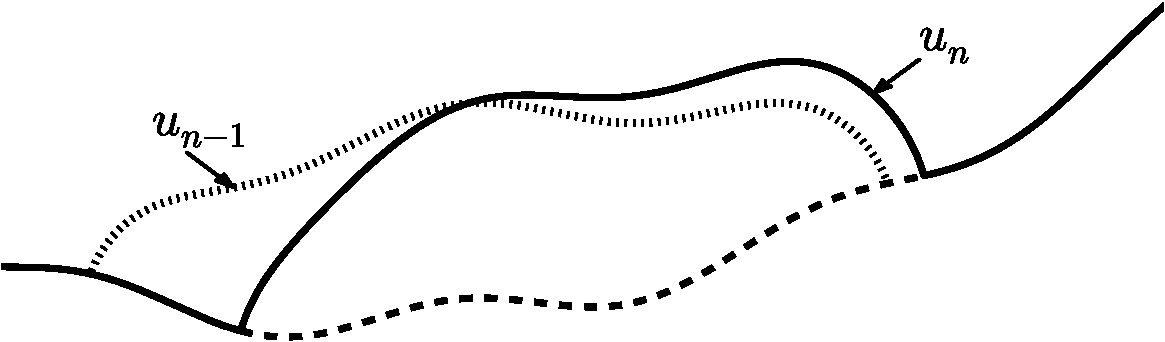
\includegraphics[width=3.9in,keepaspectratio=true]{time-step-cartoon}
\end{center}
\caption{The single time-step problem is a free boundary problem determining a new layer thickness $u_n$ from an old thickness $u_{n-1}$.}
\label{fig:timestepcartoon}
\end{figure}

Corresponding to \eqref{eq:massconserve} and \eqref{eq:constraint}, the strong form of the problem is
\begin{align}
\frac{u_n - u_{n-1}}{\Delta t} + \Div \bQ_n(\grad u_n,u_n,x) &= F_n(u_n,x) &&\text{in } \Omega, \text{ where } u_n > 0 \label{eq:semimassconserve} \\
u_n &\ge 0 &&\text{in } \overline{\Omega} \label{eq:semiconstraint}
\end{align}
In equations \eqref{eq:semimassconserve}--\eqref{eq:semiconstraint}, the semi-discretization procedure applied to \eqref{eq:massconserve} and \eqref{eq:constraint} generates the key functions
\begin{equation}
\bQ_n(\bX,v,x), \quad F_n(v,x) \label{eq:functionalforms}
\end{equation}
Here $\bX\in\RR^d$ is any vector, $v\in\RR$, and $x\in \Omega$.  We will assume $\bQ_n$ is defined for any $v\in\RR$, not just $v\ge 0$.  Furthermore, we will assume $\bQ_n$ is defined for all $x\in\Omega$, not just where $v(x)>0$, but that $\bQ_n(\bX,0,x)=0$ (subsection \ref{subsec:fluxassumptions}).

The weak form of problem \eqref{eq:semimassconserve} and \eqref{eq:semiconstraint} is stated in section \ref{sec:weakform} with attention to function spaces and well-posedness.  Though the weak form is more fundamental, both tradition and the developed intuition of practitioners suggests we should state the strong form first.  Essentially all climate-relevant literature uses the strong form rather than weak variational statements of the full free-boundary problem.

In the simplest implicit time-discretized case, namely using a backward Euler scheme applied to \eqref{eq:massconserve}--\eqref{eq:constraint}, we have $\bQ_n = \bq(\bX,v,x,t_n)$ and $F_n = f(v,x,t_n)$.  However, according to the particular discretization procedure, we intend that the source function $F_n$ ``absorbs'' all the terms, whether evaluated at $t_{n-1}$ or $t_n$, which do not involve the flux $\bq$ evaluated at time $t_n$.  For example, and including the backward Euler case above, consider a $\theta$-method discretization of \eqref{eq:massconserve} with $0\le \theta \le 1$.  The result is
\begin{align}
  &\frac{u_n - u_{n-1}}{\Delta t} + \theta\, \Div \bq(\grad u_n,u_n,x,t_n) + (1-\theta) \Div \bq(\grad u_{n-1},u_{n-1},x,t_{n-1}) \label{eq:thetamethod} \\
  &\qquad =  \theta f(u_n,x,t_n) + (1-\theta) f(u_{n-1},x,t_{n-1}). \notag
\end{align}
This is of form \eqref{eq:semimassconserve} with
\begin{align*}
\bQ_n(\bX,v,x) &= \theta\, \bq(\bX,v,x,t_n), \\
F_n(v,x)       &= \theta f(v,x,t_n) + (1-\theta) f(u_{n-1},x,t_{n-1}) \\
               &\qquad - (1-\theta) \Div \bq(\grad u_{n-1},u_{n-1},x,t_{n-1}),
\end{align*}
where the already-computed function $u_{n-1}(x)$ represents part of the dependence on $x$.  The $\theta=0$ case of \eqref{eq:thetamethod} is the forward Euler method, $\theta=1/2$ is trapezoid, and $\theta=1$ is backward Euler.  The case where $\bQ_n=0$, e.g.~from the forward Euler method, is included in our weakly-posed theory (subsection \ref{sec:weakform}).  Naturally, however, implicitness is helpful for stability and efficiency reasons.

Our theory is not limited to the $\theta$-methods.  In particular, multi-stage one-step schemes like Runge-Kutta can be put in the form of \eqref{eq:semimassconserve}---see the Appendix.  There is every reason to expect multi-step integration methods to also fit into the given framework, but the low regularity of the solution in the vicinity of the free boundary suggests caution in any expected accuracy improvements from such schemes.

\subsection{Associated set decomposition}  \label{subsec:setdecompose}  We decompose $\Omega$ using the solution of problem \eqref{eq:semimassconserve} and \eqref{eq:semiconstraint}, defining three disjoint regions based on $u_n$ and $u_{n-1}$:
\begin{align*}
\Omega_n &= \left\{x \in \Omega \,\big|\, u_n(x)>0\right\}, \\
\Omega_n^r &= \left\{x \in \Omega \,\big|\, u_n(x)=0 \text{ and } u_{n-1}(x) > 0\right\}, \\
\Omega_n^0 &= \left\{x \in \Omega \,\big|\, u_n(x)=0 \text{ and } u_{n-1}(x) = 0\right\},
\end{align*}
so that
\begin{equation}
\Omega = \Omega_n \cup \Omega_n^r \cup \Omega_n^0.  \label{eq:omegadecomposition}
\end{equation}
Here the superscript ``$r$'' stands for ``retreat,''\footnote{A symmetry has been broken, as we could have decomposed $\Omega= \Omega_{n-1} \cup \Omega_n^a \cup \Omega_n^0$ where $\Omega_{n-1}$ is the support of $u_{n-1}$ and $\Omega_n^a = \{u_n(x) > 0 \text{ and } u_{n-1}(x) = 0\}$ is the ``advance'' set.  This alternate theory offers no apparent advantages or disadvantages.} and $\Omega_n^r$ is called the \emph{retreat set}.

Figure \ref{fig:domains} shows this decomposition of $\Omega$.  Note that if $u_n$ is continuous then $\Omega_n$ is open.  If $\Omega_n$ is open then sets $\Omega_n^r \cup \Omega_n^0$ and $\Omega_n^0$ are closed in $\Omega$.

\begin{figure}[ht]
\begin{center}
\includegraphics[width=2.3in,keepaspectratio=true]{domains-fig}
\end{center}
\caption{We decompose $\Omega = \Omega_n \cup \Omega_n^r \cup \Omega_n^0$, where $\Omega_n$ the support of $u_n$, $\Omega_n^r$ is the retreat set, and $\Omega_n^0$ is the set on which both $u_{n-1}$ and $u_n$ are zero.}
\label{fig:domains}
\end{figure}

Assume $F_n(v,x)$ is continuous, and assume $u_n(x)$ is continuous and solves the strong form.  Rewrite \eqref{eq:semimassconserve} as
    $$u_n = u_{n-1} + \Delta t\, F_n - \Delta t\, \Div \bQ_n.$$
If $u_n=0$ then the terms on the right must, apparently, either sum to zero or be negative, as otherwise they should be balanced by a positive value for $u_n$.  Furthermore, at least intuitively, the flux of a zero-thickness layer should be zero, so $\bQ_n=0$ on $\Omega_n^r \cup \Omega_n^0$; see assumption \eqref{eq:Qiszero} below.  Thus, $u_{n-1}+\Delta t\, F_n \le 0$ on $\Omega_n^r \cup \Omega_n^0$.  However, because $u_{n-1}\ge 0$ and $\Delta t\ge 0$, we have these two facts
\begin{equation}
F_n(u_n,x) \le 0 \quad \text{ and } \quad u_{n-1} + \Delta t\, F_n(u_n,x) \le 0 \quad \text{ on } \Omega_n^r \cup \Omega_n^0. \label{eq:strongconditionswherezero}
\end{equation}
Note the contrapositive of \eqref{eq:strongconditionswherezero}: if $F_n(u_n,x)>0$ then $u_n(x)>0$.

The intuition behind conditions \eqref{eq:strongconditionswherezero}, which will be used in deriving the weak form, should be clear.  The source term must be sufficiently negative in a thickness-zero location where the layer was previously present (i.e.~in $\Omega_n^r$), or where it continues to be absent (in $\Omega_n^0$).  The strong form \eqref{eq:semimassconserve} and \eqref{eq:semiconstraint} of the single time-step problem is not, however, adequate for further mathematical progress.  Though PDE \eqref{eq:semimassconserve} applies on the set where its solution $u_n$ is positive (i.e.~on $\Omega_n$), and we have specified behavior, in the form of inequalities \eqref{eq:strongconditionswherezero}, on the set where $u_n=0$, we have in fact ``posed'' a problem in terms of its solution.  The next section puts us on firmer footing.


\section{Weak formulation of the single time-step problem}  \label{sec:weakform}

A strong form of a free-boundary problem, such as PDE \eqref{eq:semimassconserve} subject to inequality \eqref{eq:semiconstraint}, is inadequate because the boundary conditions satisfied by $u_n$ along the free boundary $\partial\Omega_n$ are not clear.  Also, as noted already, statements \eqref{eq:semimassconserve} and \eqref{eq:strongconditionswherezero}, while intuitively correct, apply on solution-dependent sets.  By contrast, the weak form of the single time-step problem, which we derive in this section, namely a variational inequality \cite{Friedman1982,KinderlehrerStampacchia1980} on a convex set of admissible functions, can be well-posed.  This weak form refers only to the set $\Omega$ and its boundary $\partial\Omega$.

We will state conditions on the discrete-time flux $\bQ_n$ first (subsection \ref{subsec:fluxassumptions}) so that we can then argue that a solution to the discrete-time strong problem is a solution to a certain variational inequality (subsection \ref{subsec:derivevi}); thereby we derive the weak form.  Then we show a converse, that a sufficiently-smooth solution of the weak problem solves the strong problem (subsection \ref{subsec:interior}).  Only in the next section \ref{sec:wellposed} do we address well-posedness, however, which depends on details of $\bQ_n$ which we do not need here.

\subsection{Flux assumptions} \label{subsec:fluxassumptions}  Let $p\ge 1$ and recall that $L^p (\Omega)$ is the Banach space of functions with norm $\|v\|_{L^p} = \left(\int_\Omega |v|^p\,dx\right)^{1/p}$.  The Sobolev space $W^{1,p}(\Omega)$ is the Banach space of functions $v$ with $v,\partial_1 v,\dots,\partial_d v \in L^p(\Omega)$ \cite{Evans1998}, with norm
\begin{equation}
  \|v\|_{1,p} = \left(\|v\|_{L^p}^p + \sum_i \|v\|_{L^p}^p\right)^{1/p}.  \label{eq:norm}
\end{equation}
Note that if $p>d$ then each $v\in W^{1,p}(\Omega)$ has a continuous representative \cite[``Morrey's inequality'']{Evans1998}, but otherwise $v$ may be discontinuous.  Denote by $W_0^{1,p}(\Omega)$ the closure of $C_c^\infty(\Omega)$ in $W^{1,p}(\Omega)$.

\medskip
\begin{definition}  \label{ass:std}  We say $\bQ_n$ satisfies the \emph{standard assumptions} if the following hold:  If $v \in W^{1,p}(\Omega)$ then, for $1/p + 1/q = 1$,
\begin{equation}
\bQ_n(\grad v,v,x) \in L^q(\Omega). \label{eq:QisLq}
\end{equation}
For fixed $x\in \Omega$, $\bQ_n(\bX,v,x)$ is continuous as a function of $\bX$ and $v$:
\begin{equation}
(\bX,v) \mapsto \bQ_n(\bX,v,x) \text{ is continuous on } \RR^d \times \RR.  \label{eq:Qiscontinuous}
\end{equation}
For $v \in W^{1,p}(\Omega)$, define $E_v = \left\{x\in\Omega \,\big|\, v(x) = 0\right\}$.  Then
\begin{equation}
\bQ_n(\grad v,v,x)=0 \quad \text{a.e.~on } E_v. \label{eq:Qiszero}
\end{equation}
\end{definition}

Thus we make two kinds of assumptions about the discrete-time flux, namely that $\bQ_n$ is a well-behaved function (i.e.~\eqref{eq:QisLq} and \eqref{eq:Qiscontinuous}) and
that $\bQ_n=0$ if the thickness is zero.  Assumption \eqref{eq:Qiszero} relates to the core meaning of $\bQ_n$ in \eqref{eq:semimassconserve}, namely that $\bQ_n$ is the flux of a layer with nonnegative thickness.  Note that $\grad v = 0$ a.e.~on $E_v$ by lemma A.4 in chapter II of \cite{KinderlehrerStampacchia1980}.

Regarding the source term $F_n$, we assume first that if $v\in W^{1,p}(\Omega)$ then
\begin{equation}
F_n(v(x),x) \in L^q(\Omega).  \label{eq:FisLq}
\end{equation}
Secondly we assume that $F_n$ is uniformly Lipshitz as a function of $v$: there is $L>0$ so that for all $x\in\Omega$ and $v_1,v_2 \in [0,\infty)$, we have
\begin{equation}
\left|F_n(v_1,x)-F_n(v_2,x)\right| \le L |v_1-v_2|.  \label{eq:Fislip}
\end{equation}
Thus $F_n$ is continuous as a function of $v$.

We do not require that $F_n$ be strictly increasing in $v$, which would be natural if we sought monotonicity of the variational form in the $\Delta t \to \infty$ (i.e.~steady state) limit.  See section \ref{sec:wellposed} and compare the discussion of monotonicity in  \cite{JouvetBueler2012}.

\subsection{Derivation of the variational inequality}  \label{subsec:derivevi}  To use the strong form in deriving a weak form and vice versa (section \ref{subsec:interior}), we need an extra assumption that $\bQ_n$ is smooth:  Let $S \subset \Omega$ be an open subset.  If $v\in W^{1,p}(S)$ then
\begin{equation}
\frac{\partial}{\partial x_i} \bQ_n(\grad v,v,x) \in L^q(S). \label{eq:Qissmooth}
\end{equation}

\medskip
\begin{theorem} \label{thm:strongimpliesweak} Suppose $u_n\ge 0$ and $v\ge 0$ are continuous functions on $\overline{\Omega}$ and that $\grad u_n,\grad v$ are in $L^p(\Omega)$.  Suppose that the boundaries of the sets $\Omega_n$ and $\Omega_n^r \cup \Omega_n^0$ in decomposition \eqref{eq:omegadecomposition} are all sufficiently smooth (e.g.~Lipshitz).  Suppose $u_n$ solves \eqref{eq:semimassconserve} on $\Omega_n$ and \eqref{eq:strongconditionswherezero} on $\Omega_n^r \cup \Omega_n^0$.  Suppose the function $\bQ_n(\bX,v,x)$ satisfies the standard assumptions and \eqref{eq:Qissmooth}.  Define $\bQ_n=\bQ_n(\grad u_n,u_n,x)$ and $F_n = F_n(u_n,x)$.  Then
\begin{equation}
-\int_{\Omega} \bQ_n \cdot \grad(v-u_n) \ge \int_{\Omega} \left(F_n - \frac{u_n - u_{n-1}}{\Delta t}\right) (v-u_n). \label{eq:morallytheVI}
\end{equation}
\end{theorem}

\begin{proof}  Let $w=v-u_n$.  Using decomposition \eqref{eq:omegadecomposition} and integration by parts (i.e.~divergence theorem)---here we use regularity of $\partial \Omega_n$ and $\partial(\Omega_n^r \cup \Omega_n^0)$ and assumption \eqref{eq:Qissmooth} on $S=\Omega_n$ and $S=(\Omega_n^r \cup \Omega_n^0)^\circ$---we get
\begin{align}
-\int_{\Omega} \bQ_n \cdot \grad w &= \int_{\Omega_n} (\Div \bQ_n) w - \int_{\partial \Omega_n} (\bQ_n \cdot \bn) w \label{eq:intbypartsfromstrong} \\
  &\qquad\quad + \int_{\Omega_n^r \cup \Omega_n^0} (\Div \bQ_n) w - \int_{\partial(\Omega_n^r \cup \Omega_n^0)} (\bQ_n \cdot \bn) w. \notag
\end{align}
Because $u_n$ is continuous, $u_n=0$ on $\partial \Omega_n$ and $\partial(\Omega_n^r \cup \Omega_n^0)$ so by \eqref{eq:Qiscontinuous} and \eqref{eq:Qiszero} we see that $\bQ_n=0$ on these boundaries.  Thus the boundary integrals in \eqref{eq:intbypartsfromstrong} are zero.  On the other hand, by \eqref{eq:semimassconserve} we get
\begin{equation}
-\int_{\Omega} \bQ_n \cdot \grad w = \int_{\Omega_n} \left(F_n - \frac{u_n - u_{n-1}}{\Delta t}\right) w + \int_{\Omega_n^r \cup \Omega_n^0} (\Div \bQ_n) w. \label{eq:equalitybeforeVI}
\end{equation}
By \eqref{eq:Qiszero} and \eqref{eq:Qissmooth} we have $\Div \bQ_n=0$ on $\Omega_n^r \cup \Omega_n^0$.  However, by \eqref{eq:strongconditionswherezero}, $F_n \le 0$ on $\Omega_n^r \cup \Omega_n^0$.  Since also $u_n=0$, $u_{n-1}\ge 0$, and $w = v-u_n = v \ge 0$ on $\Omega_n^r \cup \Omega_n^0$, we have
\begin{equation}
    \int_{\Omega_n^r \cup \Omega_n^0} (\Div \bQ_n) w = 0 \ge \int_{\Omega_n^r \cup \Omega_n^0} \left(F_n - \frac{u_n - u_{n-1}}{\Delta t}\right) w. \label{eq:inequalitybeforeVI}
\end{equation}
Combining \eqref{eq:equalitybeforeVI} and \eqref{eq:inequalitybeforeVI} we have \eqref{eq:morallytheVI}, which is written without decomposition \eqref{eq:omegadecomposition}.
\end{proof}

\medskip
We can now precisely define our weak problem.

\medskip
\begin{definition}  \label{def:spaces}  Fix $p>1$.  Denote $\mathcal{X} = W_0^{1,p}(\Omega)$ with norm \eqref{eq:norm} denoted by $\|\cdot\|$.  Recalling $\mathcal{X}$ is a reflexive Banach space, denote its dual space by $\mathcal{X}'$, and the pairing of $\mathcal{X}'$ and $\mathcal{X}$ by $\ip{\cdot}{\cdot}$.  Define
    $$\mathcal{K} = \left\{v \in \mathcal{X} \,\big|\, v(x) \ge 0 \text{ for all } x \in \Omega\right\}.$$
\end{definition}
It is easy to see that $\mathcal{K}$ is a closed, convex subset of $\mathcal{X}$.  

\medskip
\begin{definition}  Suppose $u_{n-1}\in\mathcal{K}$ and $\Delta t>0$.  Assume that the flux function $\bQ_n(\bX,v,x)$ satisfies \eqref{eq:QisLq} and that the source function $F_n(v,x)$ satisfies \eqref{eq:FisLq}.  Define
    $$A_n:\mathcal{K} \to \mathcal{X}'$$
by
\begin{equation}
  \ip{A_n(v)}{\phi} = \int_\Omega \left(v - \Delta t\, F_n(v,x) - u_{n-1}\right)\phi - \Delta t\, \bQ_n(\grad v,v,x) \cdot \grad\phi. \label{eq:defineAn}
\end{equation}
We can write \eqref{eq:morallytheVI} as
\begin{equation}
  \ip{A_n(u_n)}{v-u_n} \ge 0 \quad \text{for all $v \in \mathcal{K}$.}\label{eq:theVI}
\end{equation}
\end{definition}

So now the weak formulation of the single time-step problem is this:  Given $u_{n-1}\in\mathcal{K}$, solve \eqref{eq:theVI} for $u_n\in\mathcal{K}$.  Relative to the strong form, this statement both avoids using the solution to say on which subset of $\Omega$ a pointwise equality or inequality applies, and it requires much less regularity of the functions $u_{n-1}$ and $u_n$.  In section \ref{sec:wellposed}, for a variety of cases for $\bQ_n$, we will show that it determines $u_n$ uniquely, i.e.~that \eqref{eq:theVI} is a well-posed problem.

\subsection{Interior condition}  \label{subsec:interior}  We can further justify the weak form by showing a converse of Theorem \ref{thm:strongimpliesweak}.  In Theorem \ref{thm:weakimpliesstrong} below, an ``interior condition'', we need no regularity assumptions on set boundaries in decomposition \eqref{eq:omegadecomposition}.  It says that a continuous weak solution $u_n$ of \eqref{eq:theVI} solves the PDE \eqref{eq:semimassconserve} where it is positive, and otherwise it satisfies inequalities \eqref{eq:strongconditionswherezero}.

\medskip
\begin{theorem} \label{thm:weakimpliesstrong}  Assume $\bQ_n$ satisfies \eqref{eq:QisLq}, \eqref{eq:Qiscontinuous}, \eqref{eq:Qiszero}, and \eqref{eq:Qissmooth}, and assume $F_n$ satisfies \eqref{eq:FisLq}.  Suppose $u_n\in\mathcal{K}$ solves the single-time-step weak problem \eqref{eq:theVI}.
\renewcommand{\labelenumi}{\emph{(\roman{enumi})}}
\begin{enumerate}
\item If $S \subset \Omega_n$ is open, $\overline{S}\subset \Omega$, $u_n\in C(S)$, and $u_n(x)>0$ for all $x\in S$, then equation \eqref{eq:semimassconserve} applies a.e.~$x\in S$.
\item If $S \subset \Omega_n^0$ is open then $F_n \le 0$ a.e.~$x\in S$.
\item If $S \subset \Omega_n^r$ is open then $u_{n-1} + \Delta t\,F_n \le 0$ a.e.~$x\in S$.
\end{enumerate}
\end{theorem}

\medskip
\begin{proof}  To prove (i) let $\phi\in C_c^\infty(S)$ be extended by zero to all of $\Omega$; note that $\phi$ can have either sign, but that $\phi=0$ on $\partial\Omega$.  Let $v = u_n + \eps \phi$ and note that $v \in \mathcal{K}$ as long as $\eps\in\RR$ is sufficiently small in magnitude.  Specifically, $\eps$ is sufficiently small if $|\eps|\le \eps_0$ where $\eps_0 = \min u_n(x) / \max |\phi(x)| > 0$, with the minimum and maximum taken over the (compact) closure of the support of $\phi$.  It follows from variational inequality \eqref{eq:theVI} that
   $$\eps \int_\Omega \left(u_n - \Delta t\,F_n - u_{n-1}\right)\phi - \Delta t\,\bQ_n \cdot \grad \phi \ge 0.$$
This is true for all $\eps$ of either sign which are sufficiently small (i.e.~for $-\eps_0 \le \eps \le \eps_0$), so the integral is zero.  Integration by parts, using assumption \eqref{eq:Qissmooth} and $\phi\big|_{\partial\Omega}=0$, gives
   $$\int_\Omega \left[ u_n - \Delta t\,F_n - u_{n-1} + \Delta t\,\Div\bQ_n \right]\phi = 0.$$
Because $\phi\in C_c^\infty(S)$ is arbitrary, the quantity in square brackets is zero a.e., thus equation \eqref{eq:semimassconserve} applies a.e.

To prove (ii) and (iii) we start with \emph{nonnegative} $\phi\in C_c^\infty(S)$.  Again extending $\phi$ by zero to all of $\Omega$, let $v = u_n + \phi$, so $v\in\mathcal{K}$.  Because $S\subset \Omega_n^r\cup\Omega_n^0$, $u_n=0$ on the support of $\phi$.  By assumptions \eqref{eq:Qiscontinuous} and \eqref{eq:Qiszero}, $\bQ_n=0$ on the support of $\phi$ also.  Thus by \eqref{eq:theVI}, or equivalently \eqref{eq:morallytheVI},
    $$0 \ge \int_{\Omega} \left(u_{n-1} + \Delta t\, F_n\right) \phi.$$
It follows as before that $u_{n-1} + \Delta t\, F_n \le 0$ a.e.~on $S$.  In the case that also $u_{n-1}=0$ on $S$, i.e.~in case (ii), this implies $F_n \le 0$ a.e.~on $S$.\end{proof}

\medskip
From now on we will use set decomposition \eqref{eq:omegadecomposition} when referring to a solution $u_n$ of the weak form \eqref{eq:theVI}.


\section{Well-posedness for the single time-step problem} \label{sec:wellposed}  Our goal in this section is to demonstrate that a variety of different fluxes $\bQ_n$ allow a well-posed weak single time-step problem, variational inequality \eqref{eq:theVI}.  The optimistic reader, who already believes in well-posed mass conservation equation models with free boundaries, can proceed to section \ref{sec:spacediscretized} where fully-discretized, and thus implementable, numerical schemes are described.  Note, however, that the \emph{a posterior} analysis of free boundary conservation errors in section \ref{sec:timeseries} distinguishes time-semi-discretized (this section) and fully-discretized (section \ref{sec:spacediscretized}) free boundary conservation errors.

Techniques for proving well-posedness of time-independent variational inequalities in Banach spaces are relatively well-established for certain linear and some nonlinear elliptic problems.  We recall some of these tools, for monotone variational inequalities \cite{KinderlehrerStampacchia1980}, in subsection \ref{subsec:mono}, in the case where the source term $F_n$ is solution-independent.  Then in the next four subsections we prove existence and uniqueness of problem \eqref{eq:theVI} for these flux cases:
\begin{itemize}
\item[\ref{subsec:plap}] $p$-Laplacian-type parabolic (diffusion) fluxes for $1<p<\infty$;
\item[\ref{subsec:advect}] linear advection fluxes with differentiable velocity fields, with the addition of small parabolic leading-order terms;
\item[\ref{subsec:powertransform}] doubly-nonlinear parabolic fluxes including the porous medium case; and
\item[\ref{subsec:nonlocal}] linear non-local fluxes computed by integrals over $\Omega$.
\end{itemize}
In subsections \ref{subsec:plap}--\ref{subsec:nonlocal} we only consider fully-implicit (i.e.~backward Euler) time-stepping schemes.  In \ref{subsec:explicit} we see how regularity issues stop us from having the well-posed, \emph{continuous-space} single time-step free boundary problems if time-stepping is explicit or semi-explicit.  The fully-discretized schemes in section \ref{sec:spacediscretized} allow arbitrary balance between implicitness and explicitness, however.

\subsection{Monotonicity and sufficient conditions on flux for well-posedness} \label{subsec:mono}  Recall that $\mathcal{X}$ is a Banach space and $\mathcal{K}$ is a closed, convex subset of $\mathcal{X}$.  A mapping $A : \mathcal{K} \to \mathcal{X}'$ is \emph{monotone} \cite{KinderlehrerStampacchia1980} if
\begin{equation}
   \ip{A(u) - A(v)}{u-v} \ge 0  \label{eq:monodef}
\end{equation}
for all $u,v\in\mathcal{K}$.  A monotone mapping $A$ is \emph{strictly monotone} if equality in \eqref{eq:monodef} implies $u=v$.  A mapping $A$ is \emph{coercive} \cite{KinderlehrerStampacchia1980} if there is $\phi\in \mathcal{K}$ so that
\begin{equation}
   \lim_{\|u\|\to\infty} \frac{\ip{A(u) - A(\phi)}{u-\phi}}{\|u-\phi\|} = +\infty, \label{eq:coercivedef}
\end{equation}
where the limit is taken over $u\in\mathcal{K}$.  Intuitively, $A$ is coercive if the function $h(u)=\ip{A(u) - A(\phi)}{u-\phi}$ is more ``confining'' at $\infty$ than the norm $\|u-\phi\|$.

The theory of monotone variational inequalities in Banach spaces \cite[chapter III]{KinderlehrerStampacchia1980} says that the variational inequality in \eqref{eq:theVI}, i.e.
\begin{equation}
    \ip{A(u)}{v-u} \ge 0 \quad \text{for all $v\in\mathcal{K}$}, \label{eq:VIabstract}
\end{equation}
has a unique solution if $A$ is strictly monotone, coercive, and continuous on finite-dimensional subspaces.  A mapping $A : \mathcal{K} \to \mathcal{X}'$ is \emph{continuous on finite-dimensional subspaces} if for each finite-dimensional subspace $\mathcal{M} \subset \mathcal{X}$, the restriction $A : \mathcal{K}\cap \mathcal{M} \to \mathcal{X}'$ is weakly-continuous \cite{KinderlehrerStampacchia1980}.  Note that strict monotonicity by itself implies uniqueness.

For variational inequality \eqref{eq:theVI} with $A_n$ defined by \eqref{eq:defineAn} we want to relate the properties of the flux $\bQ_n$ to monotonicity and coerciveness properties of $A_n$.  An easy calculation applies in the case that $F_n=F_n(x)$, i.e.~when the source function $F_n(v,x)$ is independent of the thickness $v$:
\begin{align}
   &\ip{A_n(u) - A_n(v)}{u-v}  \label{eq:AtoQcalculation} \\
   &\qquad = \int_\Omega (u-v)^2 - \Delta t\, \left[\bQ_n(\grad u,u,x) - \bQ_n(\grad v,v,x)\right] \cdot \grad(u-v).  \notag
\end{align}
The following lemma uses the fact that $W^{1,p}(\Omega) \subset L^2(\Omega)$ if either $p>d$ or $d\le 2$; see Sobolev's lemma, theorems 5.6.2 and 5.6.5, in \cite{Evans1998}.

\begin{lemma}  \label{lem:monotonecoercive}  Suppose $\frac{1}{2} \ge \frac{1}{p} - \frac{1}{d}$.  Suppose \eqref{eq:QisLq} and that $F_n=F_n(x) \in L^q(\Omega)$.  Then

(i)  $A_n$ is (strictly) monotone if there is ($C<1$) $C\le 1$ so that
\begin{equation}
\int_\Omega \left[\bQ_n(\grad u,u,x) - \bQ_n(\grad v,v,x)\right] \cdot \grad(u-v) \le \frac{C}{\Delta t} \|u-v\|_{L^2}^2 \label{eq:Qnmonotone}
\end{equation}
for all $u,v \in \mathcal{K}$.

(ii)  $A_n$ is coercive and strictly-monotone if there is $c>0$ and $r>1$ so that
\begin{equation}
\int_\Omega \left[\bQ_n(\grad u,u,x) - \bQ_n(\grad v,v,x)\right] \cdot \grad(u-v) \le - c \|u-v\|^r \label{eq:Qncoercive}
\end{equation}
for all $u,v \in \mathcal{K}$.
\end{lemma}

Note that the right side of \eqref{eq:Qncoercive} is non-positive, and that it uses the norm in $W^{1,p}(\Omega)$.  Observe that \eqref{eq:Qncoercive} implies \eqref{eq:Qnmonotone} with $C=0$, so \eqref{eq:Qncoercive} implies strict monotonicity for $A_n$, independent of $\Delta t$.  Also, \eqref{eq:Qnmonotone} is necessary and sufficient for monotonicity of $A_n$, while \eqref{eq:Qncoercive} is merely sufficient for coercivity.  (For example, if the right side of \eqref{eq:Qncoercive} were ``$- c \|u-v\| \log \|u-v\|$'' then $A_n$ would be coercive.)

In considering lemma \ref{lem:monotonecoercive}, note that in cases where $\bQ_n(\grad u,u,x)$ is proportional to $\grad u$ we expect, for physical reasons, that the flux $\bQ_n$ points in the direction of the negative of $\grad u$.  By contrast, if $\bQ_n = \alpha \grad u$ for $\alpha>0$ then PDE \eqref{eq:massconserve} would be the ill-posed backward heat equation.

\medskip
\begin{lemma}  \label{lem:continuous}  Assume \eqref{eq:Qiscontinuous} for $\bQ_n$ and \eqref{eq:Fislip} for $F_n$.  The map $A_n$ defined by \eqref{eq:defineAn} is continuous on finite-dimensional subspaces.
\end{lemma}

\begin{proof} Choose $\{v_i\}_{i=1}^m \subset \mathcal{K}$ and let $\mathcal{M}=\operatorname{span}\left<v_i\right>$, as a subspace of $\mathcal{X}$.  Fix $\phi\in\mathcal{X}$.  The map $g:\RR^m \to \RR$ defined by
\begin{equation}
  g(c_1,\dots,c_m) = \ip{A_n\left(\sum_{i=1}^m c_i v_i\right)}{\phi}
\end{equation}
is continuous because of the linearity of the integral, \eqref{eq:Qiscontinuous}, and \eqref{eq:Fislip}.
\end{proof}

\medskip
Corollary III.1.8 of \cite{KinderlehrerStampacchia1980} now gives the following theorem.

\medskip
\begin{theorem}  \label{thm:monowellposed}  Suppose $\frac{1}{2} \ge \frac{1}{p} - \frac{1}{d}$ and $F_n=F_n(x)\in L^q(\Omega)$.  Suppose that $\bQ_n$ satisfies the standard assumptions and that condition \eqref{eq:Fislip} applies to $F_n$.  If \eqref{eq:Qncoercive} holds for $\bQ_n$ then the single time-step weak problem \eqref{eq:theVI} has a unique solution $u\in\mathcal{K}$.
\end{theorem}

\subsection{$p$-Laplacian fluxes} \label{subsec:plap}  We can immediately apply lemma \ref{lem:monotonecoercive} and theorem \ref{thm:monowellposed} to show well-posedness for some linear and non-linear parabolic cases, i.e.~where $\bq$ has the direction of $-\grad u$.  Consider the $p$-Laplacian \cite{Evans1998} flux
\begin{equation}
  \bQ_n(\grad u) = - k |\grad u|^{p-2} \grad u \label{eq:plapflux}
\end{equation}
with $1<p<\infty$.  Formula \eqref{eq:plapflux} includes the ordinary Fourier flux as the $p=2$ case.  For the proofs in this subsection we will assume $F_n=F_n(x)$ is independent of $u$, and we will need inequalities from Appendix \ref{app:pinequalities}.

If $p\ge 2$ then by \eqref{eq:pinequality} and \eqref{eq:poincare}
\begin{align}
\int_\Omega \left(\bQ_n(\grad u) - \bQ_n(\grad v)\right)\cdot (\grad u - \grad v) &= -k  \int_\Omega \left(|\grad u|^{p-2} \grad u - |\grad v|^{p-2} \grad v\right)\cdot (\grad u - \grad v) \notag \\
  &\le - \frac{k}{2^{p-2}} \int_\Omega |\grad u - \grad v|^p \notag \\
  &\le - \frac{k}{2^{p-2}\,C(\Omega,p)} \|u-v\|^p \label{eq:plapQnmono}
\end{align}
and thus \eqref{eq:Qncoercive} with $r=p$ and the given formula for $c$.  Thus the corresponding nonlinear operator $A_n$ from \eqref{eq:defineAn} is coercive and strictly-monotone, and problem \eqref{eq:theVI} is well-posed.

If $1<p<2$ then we have to work harder, and we cannot use condition \eqref{eq:Qncoercive} directly.  Returning to the nonlinear operator $A_n$ and using \eqref{eq:pinequality}, \eqref{eq:smallpbound}, and \eqref{eq:poincare} gives
\begin{align*}
  &\ip{A_n(u) - A_n(v)}{u-v} \\
  &\qquad = \|u-v\|_{L^2(\Omega)}^2 + \Delta t\,k \int_\Omega \left(|\grad u|^{p-2} \grad u - |\grad v|^{p-2} \grad v\right)\cdot (\grad u - \grad v) \\
  &\qquad \ge \|u-v\|_{L^2(\Omega)}^2 + \Delta t\,k (p-1) \int_\Omega \frac{|\grad u - \grad v|^2}{\left(|\grad u|+|\grad v|\right)^{2-p}} \\
  &\qquad \ge \|u-v\|_{L^2(\Omega)}^2 + \Delta t\,k (p-1) \frac{\|\grad u - \grad v\|_{L^p(\Omega; \RR^d)}^2}{\big\||\grad u|+|\grad v|\big\|_{L^p(\Omega)}^{2-p}} \\
  &\qquad \ge \|u-v\|_{L^2(\Omega)}^2 + B\, \frac{\|u - v\|^2}{\big\||\grad u|+|\grad v|\big\|_{L^p(\Omega)}^{2-p}}
\end{align*}
where $B = \Delta t\,k (p-1) C(\Omega,p)^{-2/p} >0$.  This shows $\ip{A_n(u) - A_n(v)}{u-v} \ge \|u-v\|_{L^2(\Omega)}^2$, so that $A_n$ is strictly-monotone.  On the other hand, fixing any $v$ with $\|\grad v\|_{L^p(\Omega;\RR^d)} >0$, we have
\begin{equation*}
\frac{\ip{A_n(u) - A_n(v)}{u-v}}{\|u-v\|} \ge B\, \frac{\|u - v\|}{\big\||\grad u|+|\grad v|\big\|_{L^p(\Omega)}^{2-p}} \to \infty
\end{equation*}
as $\|u\|\to\infty$ because $0<2-p<1$.  Therefore the limit \eqref{eq:coercivedef} applies, and so, again, $A_n$  is coercive and strictly-monotone.

We have proven the following theorem:

\medskip
\begin{theorem}  \label{thm:plapwellposed}  If $\Omega\subset \RR^d$ is bounded, $1<p<\infty$, $F_n=F_n(x)$ is independent of $u$, and $\bQ_n$ is given by \eqref{eq:plapflux} with $k>0$, then for any $\Delta t>0$, \eqref{eq:theVI} has a unique solution $u\in\mathcal{K}$.
\end{theorem}

\subsection{Advective fluxes from differentiable velocity} \label{subsec:advect}  We are interested in hyperbolic problems too.  The simplest such problems involve a flux which comes from considering a layer which is transported by a differentiable velocity field $\bX \in W^{1,\infty}(\Omega;\RR^d)$, so that
\begin{equation}
  \bQ_n(u,x) = \bX(x) u. \label{eq:advectflux}
\end{equation}

Consider conditions \eqref{eq:Qnmonotone} and \eqref{eq:Qncoercive} applied to \eqref{eq:advectflux}.  Take $u,v\in\mathcal{K}$ and compute
\begin{align}
   &\int_\Omega \left[\bQ_n(u,x) - \bQ_n(v,x)\right] \cdot \grad (u - v) = \int_\Omega \bX (u-v) \cdot \grad (u - v)   \label{eq:advectQnmono} \\
   &\qquad\qquad = \frac{1}{2}\,\int_\Omega \bX \cdot \grad (u - v)^2 = - \frac{1}{2}\,\int_\Omega \left(\Div\bX\right) (u - v)^2, \notag
\end{align}
after integrating by parts, because $u=v=0$ on $\partial \Omega$.

This result can be exploited in a couple of ways.  If the vector field is divergent, i.e.~if $\Div\bX\ge 0$, then clearly \eqref{eq:Qnmonotone} applies with $C=0$, and so $A_n$ is strictly monotone.  Otherwise, \eqref{eq:Qnmonotone} applies with $C = \frac{1}{2}\Delta t\,\|\Div\bX\|_{L^\infty(\Omega)}$, so it follows that $A_n$ is monotone if $C\le 1$, and strictly monotone if $C<1$.  Any bound on the product of $\Delta t$ and a norm of the velocity $\bX$ can be regarded as a CFL-type condition \cite{LeVeque2002}, but here the bound involves the amount by which $\bX$ is not volume-preserving.

There is no reason to suppose that the operator $A_n$ corresponding to \eqref{eq:advectflux}, defined by \eqref{eq:defineAn} as an operator from the convex subset $\mathcal{K} \subset \mathcal{X} = W_0^{1,p}(\Omega)$ to the dual $\mathcal{X}'$, is coercive.  However, if we add just a little bit of diffusion, here in the form of a $p$-Laplacian leading-order term with $p\ge 2$ for simplicity and coefficient $\eps>0$,
\begin{equation}
  \bQ_n(\grad u,u,x) = -\eps |\grad u|^p \grad u + \bX(x) u,   \label{eq:plapadvectflux}
\end{equation}
then the corresponding operator $A_n$ on $W_0^{1,p}(\Omega)$ is coercive.  In fact, combining calculations \eqref{eq:plapQnmono} and \eqref{eq:advectQnmono} gives
\begin{equation}
\int_\Omega \left[\bQ_n(u,x) - \bQ_n(v,x)\right] \cdot \grad (u - v) \le - c_0 \|u-v\|^p + c_1 \|u-v\|_{L^2(\Omega)}^2
\end{equation}
where $c_0=\eps\, 2^{2-p}/C(\Omega,p)>0$ and $c_1 = \frac{1}{2}\|\Div\bX\|_{L^\infty(\Omega)}$.  But then by \eqref{eq:AtoQcalculation} we have
\begin{equation}
\ip{A_n(u) - A_n(v)}{u-v} \ge c_0 \Delta t\, \|u-v\|^p + (1-\Delta t\,c_1) \|u-v\|_{L^2(\Omega)}^2.
\end{equation}
This proves the following theorem for the variational inequality problem in $W_0^{1,p}(\Omega)$:

\medskip
\begin{theorem}  \label{thm:plapadvectwellposed}  Suppose $\bQ_n$ is given by \eqref{eq:plapadvectflux} with $\eps>0$, $\bX \in W^{1,\infty}(\Omega;\RR^d)$, and $p\ge 2$.  If either $\Div \bX=0$ or
\begin{equation}
  \Delta t \le \frac{4}{\|\Div \bX\|_{L^\infty(\Omega)}}, \label{eq:plapadvectdtcond}
\end{equation}
then \eqref{eq:theVI} has a unique solution $u\in\mathcal{K}$.
\end{theorem}

\subsection{Doubly-nonlinear fluxes} \label{subsec:powertransform}  Now consider the doubly-nonlinear \cite{Raviart1970} flux
\begin{equation}
  \bQ_n(\grad u,u) = - k u^r |\grad u|^{p-2} \grad u \label{eq:doubleflux}
\end{equation}
where $k>0$, $r\ge 0$, and $1<p<\infty$.  This includes, as the $r=0$ case, the $p$-Laplacian \eqref{eq:plapflux}.  At the opposite extreme it includes the porous medium equation \cite{Vazquez2007}, where $p=2$ and $r=\gamma-1$ so that the flux is frequently written $- \tilde k \grad(u^\gamma)$.  Both powers are nontrivial for the diffusive shallow water equations \cite{AlonsoSantillanaDawson2008}, where $1<r<2$ and $1<p\le 2$, and for the shallow ice approximation \cite{Bueleretal2005,Calvoetal2002,JouvetBueler2012}, where $r=n+2$ and $p=n+1$ for an experimentally-determined exponent $1 < n \lesssim 4$ \cite{GoldsbyKohlstedt2001}.

Leaving the correct Sobolev space undetermined for a moment, we apply a power transformation
\begin{equation}
	u = w^m \qquad \text{ where } \quad m = \frac{p-1}{r+p-1} > 0. \label{eq:doubletransform}
\end{equation}
Straightforward calculation turns \eqref{eq:doubleflux} into
\begin{equation}
	\bQ_n(\grad w) = - K |\grad w|^{p-2} \grad w, \label{eq:doublenewflux}
\end{equation}
with $K=k m^{p-1}>0$, giving the $p$-Laplacian flux \eqref{eq:plapflux}.

Transformation  \eqref{eq:doubletransform} converts PDE \eqref{eq:semimassconserve} and \eqref{eq:doubleflux} to a $p$-Laplacian equation with additional zeroth-order terms, namely
\begin{equation}
    - K \Div\left(|\grad w|^{p-2} \grad w\right) + G(w,x) = 0  \label{eq:doubleplap}
\end{equation}
with
\begin{equation}
   G(w,x) = w^m - \Delta t\, F_n(w^m,x) - u_{n-1}. \label{eq:doubleGdefn}
\end{equation}
If $p=2$ then \eqref{eq:doubleplap} is semilinear (i.e.~linear in the highest-order term), so the transformation converts the porous medium equation into semilinear form.

Noting $u\ge 0$ if and only if $w\ge 0$ in transformation \eqref{eq:doubletransform}, define $\mathcal{X} = W_0^{1,p}(\Omega)$, and the admissible functions $\mathcal{K}\subset \mathcal{X}$, just as before in section \ref{sec:weakform}.  Define $A_n: \mathcal{K} \to \mathcal{X}'$ by
\begin{equation}
\ip{A_n(w)}{\phi} = \int_\Omega \Delta t\, K |\grad w|^{p-2} \grad w\cdot \grad \phi + G(w,x)\phi. \label{eq:doubleform}
\end{equation}
The weak formulation of \eqref{eq:doubleplap} is precisely \eqref{eq:theVI} with this $A_n$.  The following theorem uses the argument in subsection III.3 of \cite{KinderlehrerStampacchia1980}.

\medskip
\begin{theorem}
Let $1<p<\infty$ and $r\ge 0$.  Define $m$ by \eqref{eq:doubletransform}.  Suppose $G(w,x)$ defined by \eqref{eq:doubleGdefn} is in $\mathcal{X}'$ for all $w\in\mathcal{K}$, and that $G$ is nondecreasing in $w$.  Then $A_n$ in \eqref{eq:doubleform} is strictly monotone and coercive.  Thus \eqref{eq:theVI} has a unique solution $u\in\mathcal{K}$.
\end{theorem}

\begin{proof}
Suppose $p\ge 2$.  If $w,v\in\mathcal{X}$ then by \eqref{eq:pinequality} and Poincare inequality \eqref{eq:poincare},
\begin{align*}
\ip{A_n(w)-A_n(v)}{w-v} &= \int_\Omega \Delta t\, K \left(|\grad w|^{p-2} \grad w - |\grad v|^{p-2} \grad v\right) \cdot \grad (w-v) \\
  &\qquad\qquad + \left(G(w,x) - G(v,x)\right) (w-v) \\
  &\ge \frac{\Delta t\,K}{2^{p-2}} \int_\Omega |\grad (w-v)|^p + 0 \ge \frac{\Delta t\,K}{2^{p-2}\, C(\Omega,p)} \|w-v\|^p.
\end{align*}
The case $1<p<2$ follows by a trivial modification of the technique used in proving theorem \ref{thm:plapwellposed}.
\end{proof}

FIXME: of course assumptions on $G$ are assumptions on $F_n$.  if $F_n=F_n(x)$ we are done. because of $\Delta t$ we can still solve with increasing $F_n(u)$ as long as time steps are short

FIXME: major deficiency is no bedrock. compare results in \cite{JouvetBueler2012}


\subsection{Non-local dependence through an integral kernel} \label{subsec:nonlocal}   The examples so far in section \ref{sec:wellposed} are cases where the value of the flux $\bQ_n$ at $x\in\Omega$ is computed using only the values $u(x)$ and $\grad u(x)$.  The flux in realistic models is, however, often computed by solving another differential equation, for instance an energy or momentum conservation equation which is coupled to the mass-conservation equation \eqref{eq:massconserve}.  Therefore we consider fluxes that are non-local functions of the thickness $u$ and its spatial derivatives.  For simplicity we restrict to the linear case.

Let $\mathcal{X} = W_0^{1,2}(\Omega)$, a Hilbert space, and let $\mathcal{K}=\{u\in\mathcal{X}|u\ge 0\}$ as before.  Suppose $G_1(x,y), \dots, G_d(x,y)$ and $K(x,y)$ are scalar, real-valued functions in $L^2(\Omega\times \Omega)$; these will be our integral kernels.  Define
\begin{equation}
\bQ_n[u](x,t) = \int_\Omega \bG(x,y) u(y,t)\,dy - \int_\Omega K(x,y) \grad u(y)\,dy, \label{eq:nonlocaldefQn}
\end{equation}
where $\bG(x,y) = (G_1(x,y), \dots, G_d(x,y))$ is an $\RR^d$-valued function.  Note we use notation ``$\bQ_n[u]$'' to emphasize general, not just point-wise, dependence on $u$.

With flux \eqref{eq:nonlocaldefQn}, equation \eqref{eq:semimassconserve} is no longer a PDE, but rather a (linear) time-independent integro-differential equation.  That is, \eqref{eq:semimassconserve} is not a PDE in \emph{two} senses, first that it includes an integral operator and second that it is subject to the constraint $u_n\ge 0$.  We consider its weak form \eqref{eq:theVI}.

Let $A_n:\mathcal{K} \to \mathcal{X}'=\mathcal{X}$ be defined by \eqref{eq:defineAn}, but with $\bQ_n[u]$ from \eqref{eq:nonlocaldefQn} as the flux, so that
\begin{align}
    \ip{A_n(v)}{\phi} &= \int_\Omega \bigg[(v - \Delta t\,F_n + u_{n-1})\phi - \Delta t\,\left(\int_\Omega \bG(x,y) v(y)\,dy\right)\cdot \grad \phi \label{eq:nonlocaldefnAn} \\
                      &\qquad\qquad + \Delta t\,\left(\int_\Omega K(x,y) \grad v(y)\,dy\right)\cdot \grad \phi\,\bigg]\,dx. \notag
\end{align}
We need to assume $K$ is positive and bounded below \cite{PorterStirling1990} in the sense that there is $\delta>0$ so that if $\phi \in L^2(\Omega)$ then
\begin{equation}
   \int_\Omega \int_\Omega K(x,y) \phi(x) \phi(y)\,dx\,dy \ge \delta \|\phi\|_{L^2(\Omega)}^2.  \label{eq:nonlocalKpos}
\end{equation}
In particular this requires $K\ne 0$, but $K$ may have negative point values, and we require no symmetry.  Assumption \eqref{eq:nonlocalKpos} will allow us to show $A_n$ is coercive.  We can also show $A_n$ is strictly monotone if $\Delta t$ is not too large, with a bound in terms of a norm of the kernel $\bG$.

We do two preliminary calculations.  First, if $\phi\in\mathcal{X}$ then
\begin{equation}
  \int_\Omega \int_\Omega K(x,y) \grad \phi(x) \cdot \grad \phi(y)\,dx\,dy \ge \delta \|\grad\phi\|_{L^2(\Omega;\RR^d)}^2,  \label{eq:nonlocalKposRd}
\end{equation}
by $d$ applications of \eqref{eq:nonlocalKpos}.  Second, by two applications of Cauchy-Schwarz we get
\begin{equation}
\left|\int_\Omega \int_\Omega \bG(x,y) \cdot \grad \phi(x)\,\phi(y) \,dx\,dy\right|
  \le \|\bG\|_{L^2(\Omega\times\Omega;\RR^d)} \|\phi\|^2,   \label{eq:nonlocalGbound}
\end{equation}
where, by definition, $\|\bG\|_{L^2(\Omega\times\Omega;\RR^d)} = \left(\sum_{i=1}^d \left\|G_i\right\|_{L^2(\Omega \times \Omega)}^2\right)^{1/2}$.  We get the following theorem:

\begin{theorem}  \label{thm:nonlocalwellposed}  Suppose $F_n=F_n(x) \in L^2(\Omega)$ is independent of $u$, $G_i \in L^2(\Omega\times\Omega)$ for $i=1,\dots,d$, and $K \in L^2(\Omega\times\Omega)$ satisfies \eqref{eq:nonlocalKpos} with constant $\delta >0$.  If either $\bG=0$ or
\begin{equation}
  \Delta t < \frac{\delta}{C(\Omega,p)\, \|\bG\|_{L^2(\Omega\times\Omega;\RR^d)}},  \label{eq:nonlocaldtcond}
\end{equation}
where $C(\Omega,p)$ is the Poincar\'e constant in \eqref{eq:poincare}, then $A_n$ defined by \eqref{eq:nonlocaldefnAn} is coercive and strictly monotone, so variational inequality \eqref{eq:theVI} has a unique solution $u\in\mathcal{K}$.
\end{theorem}

\begin{proof}  Let $\phi=u-v$ for $u,v\in\mathcal{K}$.  By \eqref{eq:nonlocalKposRd}, \eqref{eq:nonlocalGbound}, and \eqref{eq:poincare},
\begin{align*}
\ip{A_n(u)-A_n(v)}{\phi} &\ge \|\phi\|_{L^2(\Omega)}^2 - \Delta t\,\int_\Omega \int_\Omega \bG(x,y) \cdot \grad \phi(x) \phi(y)\,dx\,dy \\
    &\qquad + \Delta t\,\int_\Omega \int_\Omega K(x,y) \grad \phi(x) \cdot \grad \phi(y)\,dx\,dy \\
    &\ge \|\phi\|_{L^2(\Omega)}^2 - \Delta t\,\|\bG\|_{L^2(\Omega\times\Omega;\RR^d)} \|\phi\|^2 + \delta \|\grad\phi\|_{L^2(\Omega;\RR^d)}^2 \\
    &\ge \|\phi\|_{L^2(\Omega)}^2 + \left(\frac{\delta}{C(\Omega,p)} - \Delta t\,\|\bG\|_{L^2(\Omega\times\Omega;\RR^d)}\right) \|\phi\|^2.
\end{align*}
The result follows from the definitions of coercivity and strict monotonicity, and condition \eqref{eq:nonlocaldtcond}.
\end{proof}

The observant reader will see a difference in the approaches in theorems \ref{thm:plapadvectwellposed} and \ref{thm:nonlocalwellposed}.  In the former the velocity $\bX$ in the hyperbolic flux $\bQ_n(u) = \bX(x) u$ was assumed to be differentiable.  Thereby an integration-by-parts gave a criterion for coercivity in terms of the norm of the divergence of $\bX$.  By constrast, in theorem \ref{thm:nonlocalwellposed} we assume only that $\bG$ is integrable, and thus the corresponding integration-by-parts, which would require integrable derivatives $\partial G_i/\partial x_j$, is not tried.  As a result, condition \eqref{eq:nonlocaldtcond} on $\Delta t$ is in some senses more severe than condition \eqref{eq:plapadvectdtcond}; for instance, \eqref{eq:nonlocaldtcond} involves both at kernel-positivity constant $\delta$ and the Poincar\'e constant.

\subsection{Explicit time-steps} \label{subsec:explicit}  Recall the $\theta=0$, fully-explicit, case of the time semi-discretization equation \eqref{eq:thetamethod}.  In weak form the problem is variational inequality \eqref{eq:theVI}, but with
    $$\bQ_n=0 \quad \text{ and } \quad F_n = - \Div \bq(\grad u_{n-1},u_{n-1},x) + f(u_{n-1},x).$$
The weak problem seeks $u\in\mathcal{K} \subset \mathcal{X}$ so that
\begin{equation}
\ip{A_n(u)}{\phi} = \int_\Omega (u - \Delta t\,F_n - u_{n-1})\phi \ge 0 \quad \text{ for all } \phi \in \mathcal{K}.  \label{eq:explicitweakstep}
\end{equation}
But the previous state $u_{n-1}$ must be regular enough so that $F_n$ is well defined, that is, so that $\Div \bq(\grad u_{n-1},u_{n-1},x) \in \mathcal{X}'$ and thus $F_n\in\mathcal{X}'$.

However, even if $F_n$ is in the dual space, the variational inequality is not elliptic.  If $\mathcal{X}=L^2(\Omega)$ then the single time step \eqref{eq:explicitweakstep} is a well-posed problem, namely a truncation problem with solution
\begin{equation}
u_n = \max\{0,u_{n-1} + \Delta t\,F_n\} \in L^2(\Omega)  \label{eq:explicittruncation}
\end{equation}
\cite[page 27]{KinderlehrerStampacchia1980}.  But this is not very helpful because $u_n \in L^2(\Omega)$ is not regular enough so that $\Div \bq(\grad u_{n-1},u_{n-1},x) \in \mathcal{X}' \in L^2(\Omega)$, even in the case where $\bq = \bX(x) u$ so that $\bq$ is zeroth-order in $u$.  In summary, for explicit steps the solution to a single weakly-posed time step is truncation \eqref{eq:explicittruncation}, but that solution cannot be expected to be regular enough to yield a well-posed problem at the next step.

On the other hand, fully-explicit and \emph{fully-discretized} numerical schemes are in widespread use for solving first-order and even second-order PDE problems.  So we return to these explicit schemes after adding spatial discretization in the next section.


\section{The fully-discretized single time-step problem}  \label{sec:spacediscretized}   A major purpose of our work is to understand time-dependent free-boundary mass conservation models through time semi-discretized form, as a sequence of spatial free-boundary problems.  We address well-posedness (section \ref{sec:wellposed}) and conservation errors at the free boundary (subsection \ref{subsec:retreatloss}) in such a continuous-space framework.  But aspects of our theory are only completed by fully-discretizing the models.  In this section we make weak assumptions about the spatial discretization, namely that there is some finite volume \cite{LeVeque2002} interpretation of the fully-discrete scheme.  Within this fully-discrete framework we will be able to say a bit more about time-step restrictions for explicit and semi-explicit schemes (subsection \ref{subsec:spaceexplicit}) so that we can tell a complete story about conservation errors at the free boundary (i.e.~subsection \ref{subsec:shellerror}).  First we set notation for a highly-generic finite volume scheme.

\subsection{Unstructured finite volume schemes} \label{subsec:spacenotation}  We restrict to $\Omega \subset \RR^d$ for $d=2,3$, and we suppose $\Omega$ is a polygon (polyhedron).  Our unstructured finite volume paradigm here assumes only that $\Omega$ is tiled by cells which are themselves polygons (Figure \ref{fig:fvmesh-notation}).  These polygonal cells can even be non-convex, and the number of edges (faces) per cell may vary.

For notation, the cells are indexed by $j\in J$.  Each cell $\omega_j$ has area (volume) $a_j$, so $\bar\Omega = \bigcup_{j\in J} \bar \omega_j$ and $|\Omega| = \sum_{j\in J} a_j$.  The edge (face) between cell $j$ and cell $k$ is indexed by a pair $(j,k)$, and it has length (area) $\ell_{(j,k)}$.  The $j$th cell has a set of edges $\mathcal{E}_j$ which contains those pairs $(j,k)$ so that $\omega_j$ and $\omega_k$ meet in an edge (face).  The set of all edges is the union $\mathcal{E} = \bigcup_{j\in J} \mathcal{E}_j$.

The representative thickness $u_n^j$ in cell $j$ is given the usual finite volume interpretation as an average, and similarly $F_n^j$ is a representative source term for the cell.
\begin{equation}
u_n^j \approx \frac{1}{a_j} \int_{\omega_j} u_n(x)\,dx, \qquad F_n^j \approx \frac{1}{a_j} \int_{\omega_j} F_n(u_n,x)\,dx.  \label{eq:fvthickness}
\end{equation}
The value $F_n^j$ is computed in some way from the geometry of cell $j$ and from as many values $\{u_n^j\}$ as necessary; the details do not matter here.

\begin{figure}[ht]
\begin{center}
% created by hand
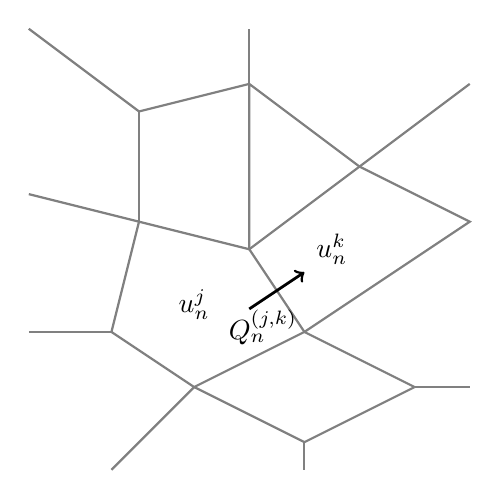
\begin{tikzpicture}[scale=0.35]
  %uncomment to see grid on which it was generated:
  %\draw[dotted,step=1.0,black,very thin] (0,0) grid (16,16);

    % exterior cell boundaries
  \draw[gray, thick] (3,0) -- (6,3);
  \draw[gray, thick] (0,5) -- (3,5);
  \draw[gray, thick] (0,10) -- (4,9);
  \draw[gray, thick] (0,16) -- (4,13);
  \draw[gray, thick] (4,13) -- (4,9);
  \draw[gray, thick] (4,13) -- (8,14);
  \draw[gray, thick] (8,14) -- (8,16);
  \draw[gray, thick] (12,11) -- (16,14);
  \draw[gray, thick] (10,5) -- (14,3);
  \draw[gray, thick] (10,1) -- (14,3);
  \draw[gray, thick] (14,3) -- (16,3);
  \draw[gray, thick] (6,3) -- (10,1);
  \draw[gray, thick] (10,0) -- (10,1);
  % interior cell boundaries
  \draw[gray, thick] (10,5) -- (8,8);
  \draw[gray, thick] (8,8) -- (12,11);



  % the free boundary is just like the other edges
  \draw[gray, thick] (6,3) -- (3,5) -- (4,9) -- (8,8) -- (8,14) --
              (12,11) -- (16,9) -- (10,5) -- cycle;
  % label some cell d.o.f.
  \draw (6,6) node {$u_n^j$};
  \draw (11,8) node {$u_n^k$};
  % show normal flux
  \def\xmid{9};
  \def\ymid{6.5};
  \def\dx{3/3};
  \def\dy{2/3};
  \draw[->,line width=1.0pt] (\xmid-\dx,\ymid-\dy) -- (\xmid+\dx,\ymid+\dy); % normal vector
  \draw (\xmid-\dx/2,\ymid-2*\dy) node {$Q_n^{(j,k)}$}; % label as flux
\end{tikzpicture}

\end{center}
\caption{Notation for a completely-unstructured finite volume mesh in $\RR^2$.}
\label{fig:fvmesh-notation}
\end{figure}

The discrete scalar normal flux across the edge $(j,k)$, outward from cell $j$, is denoted $Q_n^{(j,k)}$.  We assume that these fluxes are approximated by some scheme, based on some values $\{u_n^j\}$.  The details are not important here, but these discrete fluxes can be computed from the cell-averaged (representative) thicknesses, plus any other data, including by classical (e.g.~Gudonov) or flux-limited schemes \cite{LeVeque2002}.

We make two specific assumptions about the fully-discrete finite volume scheme:\begin{enumerate}
\item There is local conservation between any two adjacent cells which are fluid-filled:
\begin{equation}
  u_n^j u_n^k > 0 \quad \implies \quad Q_n^{(k,j)}=-Q_n^{(j,k)}.  \label{eq:fvlocalconservation}
\end{equation}
\item The strong form single-time-step problem \eqref{eq:semimassconserve} is approximated by
\begin{equation}
\frac{u_n^j - u_{n-1}^j}{\Delta t} + \frac{1}{a_j} \sum_{k\in \mathcal{E}_j} Q_n^{(j,k)} \ell_{(j,k)} = F_n^j \label{eq:fvmassconserve}
\end{equation}
in the sense that \eqref{eq:fvmassconserve} is true for each $j\in J$ such that $u_n^j > 0$.
\end{enumerate}

Local conservation (i) is completely standard, but we do not expect it at the free boundary because a flux scheme at the edge (face) of a fluid-free cell, facing a fluid-filled cell, cannot easily be expected to generate flux which is compatible with monotonicity or coercivity properties in subsection \ref{subsec:mono}, for example.  Regarding (ii), recall that, at least heuristically, the divergence of a vector field $\bX$ is the limit of line (surface) integrals, $|R|^{-1} \int_{\partial R} \bX\cdot \bn\,ds \to \Div \bX(x)$, where $R\subset \RR^d$ denotes a region with Lipshitz boundary, enclosing $x$, with outward unit normal vector $\bn$ and boundary length (area) element $ds$.  Thus the discrete scheme is assumed to approximate such an integral. 

Many schemes can be given interpretations \eqref{eq:fvthickness}--\eqref{eq:fvmassconserve}, including structured-grid (i.e.~uniform rectangular cell) finite difference \cite{MortonMayers2005} and finite volume \cite{LeVeque2002} schemes, and unstructured finite volume schemes.  Both the former structured-grid \cite{Winkelmannetal2011} and the latter unstructured-grid \cite{EgholmNielsen2010} schemes are used in ice sheet models.  A framework for unstructured-grid finite volume schemes has been implemented for ocean modeling \cite{Ringleretal2013}.  Furthermore, by considering a dual cell, the above finite volume interpretation can be applied to certain unstructured or structured finite element schemes.  Discontinuous Galerkin schemes can also be interpreted as \eqref{eq:fvmassconserve}.

\subsection{Newton-type methods for solving the single time-step variational inequality} \label{subsec:newtonvi}  FIXME: mostly generalities, but factor Jacobian into deriv of apparent stuff in \eqref{eq:theVI} and $\partial Q_n^j/\partial u_n^k$; complementarity problems \cite{BensonMunson2006,BillupsMurty2000}; example in \cite{Bueler2015}

\subsection{Fully-discrete explicit and semi-explicit schemes} \label{subsec:spaceexplicit}  FIXME:  can be well-posed but regularity concerns different


\section{\emph{A posteriori} analysis of mass conservation on the free boundary}  \label{sec:timeseries}

From now on we assume that the weak problem for a single time-step, i.e.~\eqref{eq:theVI}, is well-posed.  In particular, there is a unique sequence of states $\{u_n\}_0^N \subset \mathcal{K}$ where $N\Delta t = T$. Define
\begin{equation}
M_n = \int_\Omega u_n(x)\,dx = \int_{\Omega_n} u_n(x)\,dx, \label{eq:totalmassseries}
\end{equation}
the \emph{(total) mass} at time $t_n$, and define
\begin{equation}
C_n = \Delta t\, \int_{\Omega_n} F_n(u_n,x)\,dx, \label{eq:climateseries}
\end{equation}
the \emph{climate input} during the $n$th time step (i.e.~over the subinterval $[t_{n-1},t_n]$).  Note that the climate input $C_n$ into the fluid layer is computed by integration over locations where the fluid exists ($\Omega_n$), and not over all of $\Omega$.

Practical models of moving fluid layers would compute approximations to time-series $M_n$ and $C_n$ as model outputs, and to help a model user understand mass transfers.  A well-implemented numerical model of a fixed-boundary fluid layer problem would achieve exact discrete mass conservation in the sense that $M_n = M_{n-1} + C_n$ at each time $t_n$, to within rounding error.  One can easily show that this balance follows in the time-semi-discretized strong problem \eqref{eq:semimassconserve} if $\Omega_n=\Omega$.  Specifically, it applies under either a Neumann condition (i.e.~$\bQ_n=0$ on $\partial \Omega$) or a Dirichlet condition (i.e.~$u_n\in W_0^{1,p}(\Omega)$) under additional fluid-layer-type assumptions \eqref{eq:Qiscontinuous} and \eqref{eq:Qiszero} which force the flux to zero at the boundary (because the thickness $u_n$ goes to zero there).

\subsection{The discrete-time ``retreat loss''}  \label{subsec:retreatloss}  However, the balance $M_n = M_{n-1} + C_n$ relevant to fixed-boundary models does not follow from definitions \eqref{eq:totalmassseries} and \eqref{eq:climateseries} when there is a free boundary, that is, when $\Omega_n \subsetneq \Omega$.  Instead, recalling $\Omega_n^r$ is the retreat set in the $n$th time-step (subsection \ref{subsec:setdecompose}), define
\begin{equation}
R_n = \int_{\Omega_n^r} u_{n-1}\,dx, \label{eq:retreatlossseries}
\end{equation}
which we call the \emph{retreat loss} during the $n$th time step.  Then by \eqref{eq:semimassconserve} we have
\begin{align}
M_n - M_{n-1} &= \int_{\Omega_n} (u_n - u_{n-1})\,dx + \int_{\Omega_n^r} (0 - u_{n-1})\,dx \label{eq:newbalance} \\
   &= \Delta t \int_{\Omega_n} (- \Div \bQ_n + F_n) \,dx \, - R_n \notag \\
   &= C_n - R_n \notag
\end{align}
because $\bQ_n=0$ along $\partial \Omega_n$ by \eqref{eq:Qiscontinuous} and \eqref{eq:Qiszero}.

\subsection{The discrete-space ``shell error''}  \label{subsec:shellerror}  In the fully-discrete model, using a superscript ``$h$'' to denote the spatially-discrete version of integrated quantities, we define, analogous to \eqref{eq:totalmassseries}, \eqref{eq:climateseries}, and \eqref{eq:retreatlossseries}, respectively, the time-series
\begin{equation}
  M_n^h = \sum_j u_n^j a_j, \quad C_n^h = \Delta t\!\!\sum_{\{j:u_n^j>0\}} F_n^j a_j, \quad \text{ and } \quad R_n^h = \sum_{\{j:u_n^j=0\}} u_{n-1}^j a_j.  \label{eq:fvtimeseriesdefn}
\end{equation}
Analogous to \eqref{eq:newbalance}, by \eqref{eq:fvmassconserve} we compute
\begin{align}
M_n^h - M_{n-1}^h &= \sum_{u_n^j>0} (u_n^j - u_{n-1}^j) a_j - \sum_{u_n^j=0} u_{n-1}^j a_j \notag \\
   &= - \Delta t\,\sum_{u_n^j>0}\, \sum_{(j,k)\in\mathcal{E}_j} Q_n^{(j,k)} \ell_{(j,k)} + \Delta t\,\sum_{u_n^j>0} F_n^j a_j - \sum_{u_n^j=0} u_{n-1}^j a_j \notag \\
   &= - \Delta t\,\sum_{u_n^j>0}\, \sum_{(j,k)\in\mathcal{E}_j} Q_n^{(j,k)} \ell_{(j,k)} + C_n^h - R_n^h.  \label{eq:fvnewbalance}
\end{align}

Though in the continuous-space version \eqref{eq:newbalance} we could eliminate the flux integral, the discrete flux sum in \eqref{eq:fvnewbalance} is not zero.  Local conservation \eqref{eq:fvlocalconservation} only reduces it to a sum over edges which have a positive-thickness cell on one side and a zero-thickness cell on the other.  We call this free-boundary discrete-flux residual sum the \emph{shell error}:
\begin{equation}
S_n^h = \sum_{u_n^j>0}\, \sum_{(j,k)\in\mathcal{E}_j} Q_n^{(j,k)} \ell_{(j,k)} = \sum_{(j,k)\in\mathcal{E} \,:\, u_j^n > 0 \,\&\, u_k^n = 0} Q_n^{(j,k)} \ell_{(j,k)} \label{eq:fvderiveshellerror}
\end{equation}

\begin{figure}[ht]
\begin{center}
% created by hand
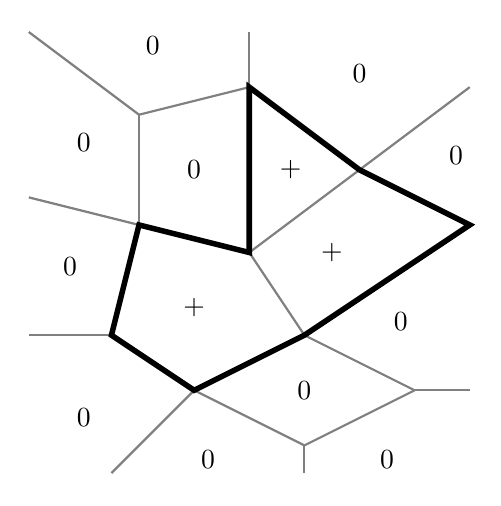
\begin{tikzpicture}[scale=0.35]
  %uncomment to see grid on which it was generated:
  %\draw[dotted,step=1.0,black,very thin] (0,0) grid (16,16);

    % exterior cell boundaries
  \draw[gray, thick] (3,0) -- (6,3);
  \draw[gray, thick] (0,5) -- (3,5);
  \draw[gray, thick] (0,10) -- (4,9);
  \draw[gray, thick] (0,16) -- (4,13);
  \draw[gray, thick] (4,13) -- (4,9);
  \draw[gray, thick] (4,13) -- (8,14);
  \draw[gray, thick] (8,14) -- (8,16);
  \draw[gray, thick] (12,11) -- (16,14);
  \draw[gray, thick] (10,5) -- (14,3);
  \draw[gray, thick] (10,1) -- (14,3);
  \draw[gray, thick] (14,3) -- (16,3);
  \draw[gray, thick] (6,3) -- (10,1);
  \draw[gray, thick] (10,0) -- (10,1);
  % interior cell boundaries
  \draw[gray, thick] (10,5) -- (8,8);
  \draw[gray, thick] (8,8) -- (12,11);



  % the free boundary is bold
  \draw[line width=2.0pt] (6,3) -- (3,5) -- (4,9) -- (8,8) -- (8,14) --
                          (12,11) -- (16,9) -- (10,5) -- cycle;
  % label cells with positive thickness
  \draw (6,6) node {$+$};
  \draw (11,8) node {$+$};
  \draw (9.5,11) node {$+$};
  % label cells with zero thickness
  \draw (2,2) node {$0$};
  \draw (1.5,7.5) node {$0$};
  \draw (2,12) node {$0$};
  \draw (4.5,15.5) node {$0$};
  \draw (6,11) node {$0$};
  \draw (12,14.5) node {$0$};
  \draw (15.5,11.5) node {$0$};
  \draw (13.5,5.5) node {$0$};
  \draw (13,0.5) node {$0$};
  \draw (6.5,0.5) node {$0$};
  \draw (10,3) node {$0$};
\end{tikzpicture}

\end{center}
\caption{The shell error $S_n^h$ is computed along those edges (strong line) where $u_n$ changes from positive (``$+$'') to zero (``$0$'').}
\label{fig:fvmesh-shellerror}
\end{figure}

As shown in Figure \ref{fig:fvmesh-shellerror}, $S_n^h$ is computed along the finite-volume approximation of the free boundary.  The quantity $S_n^h$ is an ``error'' in the sense that the continuous-space flux along the free-boundary is zero because of flux conditions \eqref{eq:Qiscontinuous}, \eqref{eq:Qiszero}.  Finally, however we can report computable time-series, namely $\{M_n^h,C_n^h,R_n^h,S_n^h\}$ which exactly balance in a fully-discrete free-boundary numerical computation:
\begin{equation}
  M_n^h = M_{n-1}^h + C_n^h - R_n^h - \Delta t\,S_n^h. \label{eq:fvfinalbalance}
\end{equation}

Furthermore, FIXME: can we \emph{show} using extensions of section \ref{sec:wellposed} technology that $R_n\to 0$ as $\Delta t\to 0$?  also assert $S_n^h\to 0$ as $h\to 0$ \emph{if} free boundary well-behaved, which is beyond scope to show, but evidently $R_n^h + \Delta t\,S_n^h \to 0$ as $\Delta t\to 0$

FIXME As an operational statement about discrete-time models, we can rephrase our major assertion from section \ref{sec:intro} as
\begin{quote}
\emph{The model must store a time series for $R_n$, in addition to the expected time series $C_n$, in order to provide auditable mass conservation.}
\end{quote}
In stating this assertion, we note that the retreat loss $R_n$ should vanish in the $\Delta t\to 0$ limit, which is a consistency statement about the time-discretized model.


\section{Conclusion} \label{sec:conclusion}

In our work, the single time-step problem is put in weak form, specifically a variational inequality (section \ref{sec:weakform}).  The nonnegativity of the thickness, $u\ge 0$, is a constraint which determines a closed, convex subset of a Banach space, the set of admissible thickness functions.  The constraint is active when negativity of the combined terms $f - \Div \bq$ in \eqref{eq:massconserve} would send the thickness below zero.  Maximum principles for the higher-order terms $\Div\bq$ in \eqref{eq:massconserve}, if applicable at all, play no role because they cannot maintain the constraint when $f<0$.  Though the form of the flux certainly affects the well-posedness, stability, and approximate-ability of the single time-step problem, our conclusions about conservation corrections at the free boundary are insensitive to the form of the flux $\bq$.

Climate-scale circulation models generally claims exact discrete conservation as a goal \cite{Thuburn2008}, but apparently always in a context without free boundary.  Such climate models are ``multiphysics'' models which generally attempt to conserve masses of the phases of water (in particular) separately, as these phases have different physical properties relevant to earth system dynamics.  For example, snow and ice have higher albedo and lower density than the liquid ocean.  In many such models, one or more fluids or phases form a layer with a moving free boundary.  We believe that auditable mass conservation does not generally occur in that case, except perhaps through \emph{ad hoc} redistribution of mass, or \emph{ad hoc} discrete schemes to locally balance the books at the free boundary.  Discrete conservation is presumably recovered in the temporal and spatial refinement limit in such models.

Thus we identify the ``retreat area'' during the time step as fundamental.  By definition this is the region where the fluid layer thickness is positive at the beginning of the time step, and, through flow and boundary-source terms, the thickness is zero at the end of the time step.  That is, fluid was completely lost from the retreat area at some time during the time-step.  Even for well-behaved source terms (e.g.~smooth in time and space) and short time steps, the retreat area can be of essentially arbitrary size.  For example, in a varying climate a large area of thin ice sheet or sea ice can melt, or a large area of a layer of surface water on ground can evaporate, and so on, during one time step.

We define the ``retreat loss'' $R_n$ as the change in mass, during the time step $[t_{n-1},t_n]$, within the retreat area.  In these terms we can answer question (ii) in the introduction more precisely:
\begin{quote}
  \emph{The retreat loss $R_n$ cannot be exactly balanced by a computable integrals of the source during the discrete time-step.}
\end{quote}
The details appear in section \ref{sec:timeseries}.  Note that the retreat losses $R_n$ goes to zero under temporal refinement even though the retreat area may not.

The above conclusions apply in the time-semi-discretized case and thus are independent of particular spatial discretization schemes.  However, in the case where the single time-step problem is well-posed in a sufficiently well-behaved Banach space (e.g.~in $W_0^{1,p}(\Omega)$; see sections \ref{sec:weakform} and \ref{sec:wellposed}), and if space is discretized using a scheme that allows a finite volume (cell-wise) mass-conservation interpretation, we identify an additional, computable free-boundary-related conservation error (subsection \ref{subsec:shellerror}).  This error $S_n$, which we call a ``shell error,'' occurs along that part of the free boundary where the flux goes to zero in the continuous case.  The shell errors $S_n$ go to zero under spatial refinement even when the time-step is not reduced.

With the conservation-correction time-series $\{R_n\}$ and $\{S_n\}$, a numerical model can ``balance the books'' exactly (i.e.~up to rounding error) in a manner which properly reflects the continuum model of the fluid layer.  A user can then assess whether these free-boundary-related conservation errors are acceptably small, just as \emph{a posteriori} estimates are used to assess whether truncation errors are acceptably small.

We believe that avoidance of, or at least clearer understanding of, \emph{ad hoc} discrete schemes to maintain conservation at free boundaries will be easier once theoretical limits on discrete conservation are acknowledged, as here.  With the proposed corrections, for example, when a large area of ice sheet or sea-ice is modeled as melting entirely in a climate simulation model, that model can measure the amount of non-conservation of the mass of water in each phase, even if that model simply transfers the ice sheet retreat loss into the ocean.  More powerfully, adaptive time-stepping schemes can be modified to reduce the retreat loss, and adaptive mesh refinement or other paradigms can reduce the shell error below prescribed tolerances.  Climate models will, in any case, be able to more-accurately report uncertainty in important mass transfers between component fluids of the climate.



%         References
\bibliography{lc}
\bibliographystyle{siam}


\appendix

\section{Inequalities for $p$-norms}   \label{app:pinequalities}  Versions of the inequality in the first Lemma \eqref{lem:pinequality} appear in the literature, at least as early as \cite{GlowinskiMarroco1975}, but here the result applies in $\RR^d$---contrast \cite{BarrettLiu1993,GlowinskiMarroco1975} for the $\RR^2$ case---and have complete proofs and explicit constants.  The proofs follow and correct those in \cite[Appendix A]{Peral1997}.

\begin{lemma}  \label{lem:pinequality}  If $1<p<\infty$ and $x,y\in\RR^n$ then
\begin{equation}
\left(|x|^{p-2} x - |y|^{p-2} y\right)\cdot(x-y) \ge
   \begin{cases}
       2^{2-p} |x-y|^p, & p\ge 2, \\
       (p-1)\, |x-y|^2 \, \left(|x|+|y|\right)^{p-2}, & 1 < p \le 2.
   \end{cases} \label{eq:pinequality}
\end{equation}
\end{lemma}

\begin{proof}  \underline{Case $p \ge 2$:}  The case where $x=0$ or $y=0$ is trivial, so assume, by swapping $x$ and $y$ as necessary, that $0 < |y| \le |x|$.  Define $t=|y|/|x|$ and $s = (x\cdot y)/(|x||y|)$ so that $0\le t \le 1$ and $|s|\le 1$.  Expand \eqref{eq:pinequality} and divide it by $|x|^p$, to get the equivalent statement
    $$1 - (t^{p-1}+t) s + t^p \ge 2^{2-p} \left(1 - 2 s t + t^2\right)^{p/2}.$$
Thus we are trying to prove that $2^{2-p}$ is a lower bound for
	$$f(t,s) = \frac{1 - (t^{p-1}+t) s + t^p}{\left(1 - 2 s t + t^2\right)^{p/2}}.$$
Note $s=1$ if and only if $x=y$, and in that case \eqref{eq:pinequality} is true.  We find a lower bound of $f$ on $(t,s) \in R=[0,1]\times[-1,1)$.  Note $1-2st+t^2 > 0$ on $ R$, so $f(t,s)$ is well-defined and differentiable on $R$.

Now, $f(t,-1) = \left(1 + t^{p-1}\right) / \left(1 + t\right)^{p-1}$ on $t\in[0,1]$.  Because $h(t)=t^{p-1}$ is convex for $p \ge 2$,
    $$\frac{1}{2^{p-1}} (1+t)^{p-1} = h(\tfrac{1}{2} 1 + \tfrac{1}{2} t) \le \tfrac{1}{2} h(1) + \tfrac{1}{2} h(t) = \tfrac{1}{2} (1 + t^{p-1}),$$
and thus $f(t,-1) \ge 2^{2-p}$.  On the other hand, a quick calculation shows
    $$\frac{\partial f}{\partial s} = \frac{t}{\left(1 - 2 s t + t^2\right)^{(p+2)/2}} g(t,s)$$
where
    $$g(t,s) = s(2-p) t (t^{p-2} + 1) + (p-1) (t^p+1) - t^{p-2} - t^2$$
is continuous on the closed rectangle $\bar R = [0,1]\times[-1,1]$.  We will show $g(t,s)\ge 0$ on $\bar R$, thus that $\partial f/\partial s \ge 0$ on $R$, and thus that $f(t,s)\ge f(t,-1) \ge  2^{2-p}$ on $R$.

Now,
    $$\frac{\partial g}{\partial s} = (2-p) t (t^{p-2} + 1) \le 0$$
on $\bar R$.  Define $G(t) = g(t,1)$.  We will show $G(t)\ge 0$ on $[0,1]$, thus that $g(t,s)\ge g(t,1)\ge 0$ on $\bar R$.  But
\begin{align*}
G(t) &\ge 0 &\iff && (2-p) t (t^{p-2} + 1) + (p-1) (t^p+1) - t^{p-2} - t^2 \ge 0 \\
          & &\iff && (p-1) (t-1) (t^{p-1}-1) \ge (t^{p-2} - t) (1 - t)  \\
          & &\iff && (p-1) (1 - t^{p-1}) \ge t^{p-2} - t.
\end{align*}
Note $(p-1) (1 - t^{p-1}) \ge 0$.  If $p\ge 3$ then $t^{p-2} - t \le 0$ so $G(t)\ge 0$ in that case.  On the other hand, if $2\le p < 3$ then
	$$\frac{t^{p-2} - t}{1 - t^{p-1}} = t^{p-2} \frac{1 - t^{3-p}}{1 - t^{p-1}} \le t^{p-2} \le 1 \le p-1$$
on $t\in[0,1)$, because $t^{p-1}\le t^{3-p}$ and thus $1 - t^{p-1} \ge 1 - t^{3-p}$.  But also $G(1)=0$, so $G(t)\ge 0$ on $[0,1]$.

\medskip
\noindent \underline{Case $1 < p \le 2$:}  Assuming $x,y$ are not both zero, by symmetry (swapping $x$ and $y$) and homogeneity (replacing $x,y$ with $\lambda x,\lambda y$) we can assume $|x| = 1 \ge |y|$.  Furthermore, by choosing a basis of $\RR^n$ we can have $x=(1,0,\dots,0)$ and $y=(y_1,y_2,0,\dots,0)$ where $y_1^2+y_2^2 \le 1$.  In these terms, the inequality we seek to prove is
\begin{align*}
&\left(1 - (y_1^2+y_2^2)^{\frac{p-2}{2}} y_1\right) (1-y_1) + (y_1^2+y_2^2)^{\frac{p-2}{2}} y_2^2 \\
&\qquad\qquad \ge (p-1)\, \left((1-y_1)^2+y_2^2\right) \left(1 + \sqrt{y_1^2+y_2^2} \right)^{p-2}.
\end{align*}
(Compare equation (A.4) in \cite{Peral1997}.)  But
\begin{align*}
1 - (y_1^2+y_2^2)^{\frac{p-2}{2}} y_1
      &\ge \begin{cases} 1-y_1, & y_1 \le 0, \\
                        1-y_1^{p-1}, & 0 \le y_1 \le 1 \end{cases}\Bigg\}
      \ge (p-1) (1-y_1).
\end{align*}
(The lower case in the last inequality is easy to prove by the mean-value-theorem applied to $\varphi(t)=t^{p-1}$, for which $\varphi'(1)=p-1$ is the minimum value of the derivative on $t\in[0,1]$.)  Also noting $(y_1^2+y_2^2)^{\frac{p-2}{2}} \ge 1$ and $\left(1 + \sqrt{y_1^2+y_2^2} \right)^{2-p} \ge 1$, because $|y|\le 1$ and $p-2\le 0$, thus
\begin{align*}
&\frac{\left(1 - (y_1^2+y_2^2)^{\frac{p-2}{2}} y_1\right) (1-y_1) + (y_1^2+y_2^2)^{\frac{p-2}{2}} y_2^2}
      {\left((1-y_1)^2+y_2^2\right) \left(1 + \sqrt{y_1^2+y_2^2} \right)^{p-2}} \\
&\qquad \ge \frac{(p-1) (1-y_1)^2 + y_2^2}
      {(1-y_1)^2+y_2^2} \,  \left(1 + \sqrt{y_1^2+y_2^2} \right)^{2-p} \\
&\qquad \ge \frac{(p-1) (1-y_1)^2 + (p-1) y_2^2}{(1-y_1)^2+y_2^2} = p-1.
\end{align*}
This proves \eqref{eq:pinequality} in the case $1<p\le 2$.
\end{proof}

We will also need the result of combining the $1<p\le 2$ case of Lemma \ref{lem:pinequality}, a point-wise result, with integration over a set $\Omega$.

\begin{lemma} \label{lem:smallpbound}  Suppose $1<p\le 2$.  If $\Omega \subset \RR^d$ is measurable and if $\bu,\bv\in L^p(\Omega; \RR^m)$ for $m\ge 1$, then
\begin{equation}
    \int_\Omega \frac{|\bu-\bv|^p}{\left(|\bu|+|\bv|\right)^{2-p}} \ge \frac{\|\bu-\bv\|_{L^p(\Omega; \RR^m)}^2}{\big\||\bu|+|\bv|\big\|_{L^p(\Omega)}^{2-p}}. \label{eq:smallpbound}
\end{equation}
\end{lemma}

\begin{proof}  By H\"older inequality with $r=2/p$ and $s=2/(2-p)$, so $r^{-1}+s^{-1}=1$,
\begin{align*}
\int_\Omega |\bu - \bv|^p &= \int_\Omega \frac{|\bu-\bv|^p}{\left(|\bu|+|\bv|\right)^{p(2-p)/2}} \left(|\bu|+|\bv|\right)^{p(2-p)/2} \\
    &\le \left(\int_\Omega \frac{|\bu-\bv|^2}{\left(|\bu|+|\bv|\right)^{2-p}}\right)^{p/2} \left(\int_\Omega \left(|\bu|+|\bv|\right)^p\right)^{(2-p)/2},
\end{align*}
thus \eqref{eq:smallpbound}.
\end{proof}

Finally we recall the classical Poincar\'e inequality on the Sobolev space $W_0^{1,p}(\Omega)$, which is defined at the beginning of subsection \ref{subsec:fluxassumptions}.  The form of the Poincar\'e inequality in the following Lemma, with an explicit but not optimal constant, is from \cite[section 7.8]{GilbargTrudinger2001}.

\begin{lemma} \label{lem:poincare}  If $\Omega\subset \RR^d$ is a bounded domain with volume $|\Omega|$, and if $1\le p<\infty$ then for all $u\in W_0^{1,p}(\Omega)$,
\begin{equation}
  \|u\|_{W^{1,p}(\Omega)}^p \le C(\Omega,p) \int_\Omega |\grad u|^p, \label{eq:poincare}
\end{equation}
where $C(\Omega,p)=1+(|\Omega|/\omega_d)^{p/d}$ and $\omega_d=(2 \pi^{d/2})/(d\,\Gamma(d/2))$ is the volume of the unit ball in $\RR^d$.
\end{lemma}


\section{Second-order Runge-Kutta time-discretization}   \label{app:rk2}  In Section \ref{sec:strongform} we describe the time semi-discretization of the continuum strong form \eqref{eq:massconserve}--\eqref{eq:constraint} using the $\theta$ method, thus including the Euler, backward Euler, and trapezoidal rules.  These one-stage time-discretizations generate particular forms for functions $\bQ_n(\bX,v,z)$ and $F_n(v,z)$ in equations \eqref{eq:semimassconserve}--\eqref{eq:semiconstraint}, and these functions define the single-time-step variational inequality problem \eqref{eq:theVI}.  In this Appendix we illustrate how these functions can be generated for certain Runge-Kutta (RK) schemes, although in some cases at the cost of having to solve multiple problems of type \eqref{eq:theVI} at each time step.  Higher-order RK schemes can be handled without any additional ideas, but we limit our presentation to two-stage schemes for simplicity.

For the $m$-dimensional ODE system
\begin{equation}
  \by' = \bbf(t,\by),  \label{eq:abstractODE}
\end{equation}
every two-stage RK scheme with time-step $h=\Delta t$ can be written with Butcher tableau \cite{AscherPetzold1998}
\begin{equation}
\begin{array}{c|cc}
\tau_1 & a_{11} & a_{12}  \\
\tau_2 & a_{21} & a_{22}  \\ \hline
       & b_1    & b_2     \\
\end{array}  \label{eq:tableau}
\end{equation}
representing the formulas
\begin{align*}
  \by_{n,i} &= \by_{n-1} + h \sum_{j=1}^2 a_{ij} \bbf(t_{n-1} + \tau_j h, \by_{n,j}), \\
      \by_n &= \by_{n-1} + h \sum_{i=1}^2 b_i \bbf(t_{n-1} + \tau_i h, \by_{n,i}),
\end{align*}
with $i=1,2$ in the first equation.  \emph{Explicit} methods have $a_{ij}=0$ for $j\ge i$ (i.e.~zeros on and above the diagonal) and, by definition, \emph{semi-implicit} methods have $a_{12}=0$.  We consider only explicit and semi-implicit methods in this paper.  For example, the $\theta$-methods used in Section \ref{sec:strongform} have tableau
\begin{equation*}
\begin{array}{c|cc}
0 &          &   \\
1 & 1-\theta & \theta  \\ \hline
  & 1-\theta & \theta  \\
\end{array}
\end{equation*}
when written as a two-stage scheme.  Note that $\theta>0$ methods are semi-implicit but not diagonally-implicit.

So-called (singly) \emph{diagonally-implicit} RK (``DIRK'') methods are semi-implicit methods for which the diagonal entries $a_{ii}$ are independent of $i$, i.e.~$a_{11}=a_{22}$.  The accuracy of $s$-stage DIRK methods is limited to $p=s+1$ \cite{AscherPetzold1998}.  There exist strongly S-stable and stiffly-accurate \cite{AscherPetzold1998} DIRKs with $s$ stages and order of accuracy $p=s$ for $s=1,2,3$ \cite{Alexander1977}.  Note that ``strongly S-stable'' is also called ``stiff decay'' \cite{AscherPetzold1998}.

The strong stability properties of these DIRK methods are exactly what is needed for many of the applications addressed in the current paper, namely diffusive cases where $\bq \sim - \grad u$.  In these diffusive cases the $m$-dimensional method-of-lines ODE system generated by spatially-semi-discretizing \eqref{eq:massconserve} would become arbitrarily stiff under spatial refinement.  Furthermore, semi-implicit methods have the computational advantage, especially in our large $m$ case arising from discretization of a PDE, that each stage represents a separate linear system of only $m$ equations to solve.  (General $s$-stage implicit RK schemes require solving size $sm$ linear systems, but for semi-implicit RK schemes the matrix has block lower-triangular form.)  DIRK methods have the further advantage that the $m\times m$ matrix $A$ for each stage $i$, or the Jacobian matrix arising from the linearization of the stage, can be re-used at each stage during a step. In fact the matrix has $i$-independent form $A = I - h a_{ii} J$, at least if the Jacobian $J$ is evaluated at only at the start of the time step in the nonlinear case: $J = \frac{\partial \bbf}{\partial y}(t_{n-1},\by_{n-1})$.

Functions $\bQ_n$ and $F_n$ in \eqref{eq:functionalforms} are needed to state the weak problem \eqref{eq:theVI}.  We compute these functions for two particular DIRK schemes, the $(s,p)=(1,2)$ A-stable scheme known as the implicit midpoint rule, and the unique strongly S-stable $(s,p)=(2,2)$ scheme for which $0\le \tau_i\le 1$.  The significance of the latter condition on $\tau_i$ for our context is that the source term $f$ in \eqref{eq:massconserve} is only evaluated at $t$ in the interval $[t_{n-1},t_n]$ when computing $u_n$; the other strongly S-stable $(s,p)=(2,2)$ method, oddly enough, has $\tau_1>1$.

\begin{itemize}
\item We write the implicit midpoint rule as a two-stage scheme with tableau
\begin{equation*}
\begin{array}{c|cc}
0           &    &             \\
\frac{1}{2} & 0  & \frac{1}{2} \\ \hline
            & 0  & 1           \\
\end{array}
\end{equation*}
This scheme has two equations: the first stage is a backward Euler step of $\frac{1}{2} h$, but the second stage is explicit.  Using the notation $\tilde\by = \by_{n,2}$ for the scheme applied to ODE system \eqref{eq:abstractODE}, the equations are
\begin{align}
\tilde\by &= \by_{n-1} + \tfrac{1}{2} h \bbf(t_{n-1}+\tfrac{1}{2}h,\tilde\by), \label{eq:impmida} \\
\by_n &= \by_{n-1} + h \bbf(t_{n-1}+\tfrac{1}{2}h,\tilde\by). \label{eq:impmidb}
\end{align}

Let $t_{n-1/2} = t_{n-1} + \tfrac{1}{2} \Delta t$ using the notation of the main paper.  Then the functions \eqref{eq:functionalforms} for the first stage \eqref{eq:impmida} are
  $$\tilde\bQ(\bX,v,x) = \tfrac{1}{2} \bq(\bX,v,x,t_{n-1/2}) \quad \text{and} \quad \tilde F(v,x) = \tfrac{1}{2} f(v,x,t_{n-1/2}).$$
The functions for the second stage \eqref{eq:impmidb} are
  $$\bQ_n(\bX,v,x) = 0$$
and
  $$\quad F_n(v,x) = f(\tilde u,x,t_{n-1/2}) - \Div \bq(\grad\tilde u,\tilde u,x,t_{n-1/2})$$
where $\tilde u$ denotes the weak solution to the first stage.  Neither of these second-stage functions actually depend on the unknown $v$ because stage \eqref{eq:impmidb} is explicit once \eqref{eq:impmida} is computed.
\item The strongly S-stable $(2,2)$ scheme has tableau
\begin{equation*}
\begin{array}{c|cc}
\alpha & \alpha   &        \\
1      & 1-\alpha & \alpha \\ \hline
       & 1-\alpha & \alpha \\
\end{array}
\end{equation*}
where $\alpha = (2-\sqrt{2})/2 \approx 0.293$.  Noting the stiffly-accurate condition, namely $a_{2j}=b_j$ for $j=1,2$, this scheme also has only two equations, both implicit.  Now using notation $\tilde\by = \by_{n,1}$, the stages are
\begin{align}
\tilde\by &= \by_{n-1} + \alpha h \bbf(t_{n-1}+\alpha h,\tilde\by), \label{eq:sstabledirka} \\
\by_n &= \by_{n-1} + (1-\alpha) h \bbf(t_{n-1}+\alpha h,\tilde\by) + \alpha h \bbf(t_n,\by_n). \label{eq:sstabledirkb}
\end{align}

Let $t_{n;\alpha} = t_{n-1} + \alpha \Delta t$.  The functions \eqref{eq:functionalforms} for the first stage \eqref{eq:sstabledirka} are
  $$\tilde\bQ(\bX,v,x) = \alpha \bq(\bX,v,x,t_{n;\alpha}) \quad \text{and} \quad \tilde F(v,x) = \alpha f(v,x,t_{n;\alpha}).$$
The functions for the second stage \eqref{eq:sstabledirkb} are
   $$\bQ_n(\bX,v,x) = \alpha \bq(\bX,v,x,t_n)$$
and
   $$F_n(v,x) = (1-\alpha) f(\tilde u,x,t_{n;\alpha}) + \alpha f(v,x,t_n) - (1-\alpha) \Div \bq(\grad\tilde u,\tilde u,x,t_{n;\alpha})$$
where $\tilde u$ denotes the weak solution to the first stage.
\end{itemize}

\end{document}
